\documentclass[11pt,reqno]{amsart}

\usepackage[utf8]{inputenc}
\usepackage[T1]{fontenc}
\usepackage{lmodern}
\usepackage{amsmath,amssymb,amsfonts,amsthm,mathtools}
\usepackage{booktabs,array,multirow}
\usepackage{graphicx}
\usepackage{enumitem}
\usepackage[margin=1.0in]{geometry}
\usepackage{microtype}
\usepackage{xcolor}
\definecolor{linkblue}{rgb}{0.0,0.2,0.6}
\usepackage[colorlinks=true,linkcolor=linkblue,citecolor=linkblue,urlcolor=linkblue]{hyperref}

\newtheorem{theorem}{Theorem}[section]
\newtheorem{proposition}[theorem]{Proposition}
\newtheorem{lemma}[theorem]{Lemma}
\newtheorem{corollary}[theorem]{Corollary}
\theoremstyle{definition}
\newtheorem{definition}[theorem]{Definition}
\theoremstyle{remark}
\newtheorem{remark}[theorem]{Remark}

\numberwithin{equation}{section}
\allowdisplaybreaks

\newcommand{\R}{\mathbb{R}}
\newcommand{\C}{\mathbb{C}}
\newcommand{\N}{\mathbb{N}}
\newcommand{\Z}{\mathbb{Z}}
\newcommand{\dd}{\mathrm{d}}
\newcommand{\ee}{\mathrm{e}}
\newcommand{\ii}{\mathrm{i}}
\newcommand{\Rea}{\mathrm{Re}}
\newcommand{\Ima}{\mathrm{Im}}
\newcommand{\sinch}{\mathrm{sinc}_{\mathrm{hyp}}}
\newcommand{\fac}{\mathclose{\mathchar"0021}}

\title[Second-Order De~Branges Kernels and $d=0$ Lehmer Lifting]{Second-Order Hermite--Biehler De~Branges Kernels, the Derivative-Wronskian Splitting $K_{\alpha,\beta} \equiv \frac{\alpha}{\pi}\widetilde{W}_{0,1} + \frac{\alpha\beta}{\pi}\widetilde{W}_{1,2}$, and $d=0$ Lifting of the Lehmer Near-Coalescence Degeneracy for Riemann's $\Xi$-Function}

\author{Thijs Missiaen}
\address{Independent Researcher, Belgium}
\email{thijs.missiaen@gmail.com}
\thanks{ORCID: \href{https://orcid.org/0009-0007-3678-0810}{0009-0007-3678-0810}}

\subjclass[2020]{Primary 11M06, 11M26; Secondary 30D15, 46E22}
\keywords{Riemann $\Xi$-function, transverse Wronskian, de~Branges reproducing kernel, Hermite--Biehler polynomials, Lucas--Jensen derivative Wronskian, Lehmer pairs, Hurwitz polynomials, Wigner phase-space distribution, radial Laplace PDE}
\dedicatory{\upshape October 25, 2026}
\date{October 25, 2026}

\begin{document}
\sloppy

\begin{abstract}
We prove that for the second-order Hermite--Biehler structure function $E_{\alpha,\beta}(z) := \Xi(z) - \ii\alpha\Xi'(z) - \beta\Xi''(z)$ ($\alpha > 0, \beta > 0$) studied by Lagarias, Ki, and Suzuki, the de~Branges kernel $K_{\alpha,\beta}(t-\ii d, t-\ii d)$ exhibits an exact cancellation of all three squared moduli ($|\Xi|^2, \alpha^2|\Xi'|^2, \beta^2|\Xi''|^2$) and of the $(0,2)$ cross-term $-2\beta\Rea(\overline{\Xi}\Xi'') \equiv 0$, splitting into $K_{\alpha,\beta}(t-\ii d, t-\ii d) \equiv \frac{\alpha}{\pi}\widetilde{W}_{0,1}(d,t) + \frac{\alpha\beta}{\pi}\widetilde{W}_{1,2}(d,t)$, where $\widetilde{W}_{1,2}(d,t) = \frac{1}{2d}\partial_d|\Xi'(t-\ii d)|^2$ is the parity-reduced derivative Wronskian. Consequently, as $d \to 0^+$, $\pi K_{\alpha,\beta}(t,t) \equiv \alpha c_1(t) + \alpha\beta c_1^{(1)}(t)$, so at the midpoint $t_{\mathrm{mid}}$ of any closely spaced Lehmer pair ($\Xi'(t_{\mathrm{mid}}) = 0$), $\pi K_{\alpha,\beta}(t_{\mathrm{mid}}, t_{\mathrm{mid}}) \equiv -\alpha\Xi(t_{\mathrm{mid}})\Xi''(t_{\mathrm{mid}}) + \alpha\beta(\Xi''(t_{\mathrm{mid}}))^2 \to +\alpha\beta(\Xi''(t_0))^2 > 0$ remains strictly positive on $d = 0$ at order $d^0$. Finally, we prove the radial four-dimensional Laplace coupling $\widetilde{W}_{1,2} \equiv \frac{1}{4}(\partial_d^2 + \frac{2}{d}\partial_d + \partial_t^2)\widetilde{W}_{0,1}$, the dipole recursion $c_{2m-1}^{(1)}(t) \equiv \frac{1}{4}(2m(2m+1)c_{2m+1}(t) + c_{2m-1}''(t))$, and the order-$M$ Hurwitz coalescence law $\pi K_{\boldsymbol{\alpha}}(t_0, t_0) = +\alpha_{m-1}\alpha_m(\Xi^{(m)}(t_0))^2 + \mathcal{O}(\alpha_{>m}) > 0$.
\end{abstract}

\maketitle

\section{Introduction and Main Results}\label{sec:intro}

In the analytic theory of Hilbert spaces of entire functions~\cite{debranges1968,debranges1986,debranges1992} associated with Riemann's completed zeta function $\Xi(z) := \xi(\frac{1}{2} + \ii z)$ ($z = t - \ii d$, $s = \frac{1}{2} + d + \ii t$)~\cite{riemann1859,polya1926,titchmarsh1986}, a central role is played by canonical Hermite--Biehler structure functions obtained by applying differential polynomials to $\Xi(z)$~\cite{lagarias2006,ki2008,suzuki2011}. While Conrey and Li~\cite{conreyli2000} demonstrated that global inner-product positivity conditions on classical Sonine--de~Branges spaces fail for $\xi(s)$, Lagarias~\cite{lagarias1999,lagarias2006}, Ki~\cite{ki2008}, and Suzuki~\cite{suzuki2011} investigated the direct Hermite--Biehler hierarchy generated by linear, quadratic, and higher-order differential operators:
\begin{equation}\label{eq:intro_E_alpha_beta}
E_\alpha(z) := \Xi(z) - \ii\alpha\,\Xi'(z), \qquad E_{\alpha,\beta}(z) := \Xi(z) - \ii\alpha\,\Xi'(z) - \beta\,\Xi''(z) \qquad (\alpha > 0,\; \beta > 0),
\end{equation}
including the canonical repeated-root family $E_{\alpha,\alpha^2/4}(z) = (1 - \frac{\ii\alpha}{2}\partial_z)^2\Xi(z)$ ($\beta = \alpha^2/4$).

In Paper~IV of this series~\cite{missiaen2026paper4} (building on Papers~I--III~\cite{missiaen2026paper1,missiaen2026paper2,missiaen2026paper3}), we proved that for the first-order family ($\beta = 0$), the de~Branges reproducing kernel on the diagonal $w = t - \ii d$ collapses to $K_\alpha(w,w) \equiv \frac{\alpha}{\pi}\widetilde{W}_{0,1}(d,t)$, where $\widetilde{W}_{0,1}(d,t) := \frac{1}{2d}\partial_d|\Xi(t-\ii d)|^2 = d^{-1}\Ima(\overline{\Xi(w)}\Xi'(w))$ is the parity-reduced transverse Wronskian~\cite{speiser1934,hinkkanen1997,csordas1986,griffin2019}. Although this identity decouples local off-critical zero exclusion from the global Sonine obstructions of Conrey and Li~\cite{conreyli2000}, the first-order kernel $K_\alpha(w,w)$ exhibits a structural degeneracy on the critical line $d = 0$ itself whenever two zeros approach coalescence~\cite{lehmer1956}: at a hypothetical double zero $t_0 \in \R$ ($\Xi(t_0) = \Xi'(t_0) = 0$, $\Xi''(t_0) \neq 0$), the critical-line value $\pi K_\alpha(t_0, t_0) = \alpha((\Xi'(t_0))^2 - \Xi(t_0)\Xi''(t_0)) = \alpha c_1(t_0) = 0$ vanishes at order $d^0$, so strict positivity emerges only transversely at order $d^2$ via $c_3(t_0) = \frac{1}{2}(\Xi''(t_0))^2 > 0$. Equivalently, at the critical-line extremum $t_{\mathrm{mid}}$ ($\Xi'(t_{\mathrm{mid}}) = 0$) between a closely spaced Lehmer pair $t_\pm = t_{\mathrm{mid}} \pm \delta$ ($\delta \to 0$), the first-order barrier $\pi K_\alpha(t_{\mathrm{mid}}, t_{\mathrm{mid}}) = -\alpha\Xi(t_{\mathrm{mid}})\Xi''(t_{\mathrm{mid}}) = \mathcal{O}(\delta^2) \to 0$ becomes arbitrarily small on $d = 0$.

The purpose of the present paper (Paper~XIII, continuing Papers~I--X~\cite{missiaen2026paper1,missiaen2026paper2,missiaen2026paper3,missiaen2026paper4,missiaen2026paper5,missiaen2026paper6,missiaen2026paper7,missiaen2026paper8,missiaen2026paper9,missiaen2026paper10}) is to prove that passing to the second-order Lagarias--Ki--Suzuki structure function $E_{\alpha,\beta}(z)$ ($\beta > 0$) resolves this $d = 0$ near-coalescence degeneracy completely at order $d^0$, without introducing any cross-term contamination into the reproducing kernel. Our main results are consolidated in the following theorem.

\begin{theorem}[Second-Order De~Branges Splitting, $d=0$ Lehmer Lifting, Radial Laplace Recursion, and Order-$M$ Hurwitz Chains]\label{thm:main}
Let $z = t - \ii d \in \C$ with $d \in \R \setminus \{0\}$ and $t \in \R$, and let $E_{\alpha,\beta}(z) := \Xi(z) - \ii\alpha\Xi'(z) - \beta\Xi''(z)$ and $E_{\alpha,\beta}^\#(z) := \overline{E_{\alpha,\beta}(\bar{z})} = \Xi(z) + \ii\alpha\Xi'(z) - \beta\Xi''(z)$ for $\alpha > 0, \beta > 0$. Then:
\begin{enumerate}[label=\textup{(\roman*)},leftmargin=2.2em]
\item \textbf{Exact Cross-Term-Free Second-Order De~Branges Splitting and Cauchy--Pick Decomposition.} In the numerator $|E_{\alpha,\beta}(t-\ii d)|^2 - |E_{\alpha,\beta}^\#(t-\ii d)|^2$, all three quadratic norms $|\Xi|^2$, $\alpha^2|\Xi'|^2$, and $\beta^2|\Xi''|^2$ as well as the $(0,2)$ cross-term $-2\beta\Rea(\overline{\Xi}\Xi'') \equiv 0$ cancel identically, yielding the exact global decomposition
\begin{equation}\label{eq:intro_second_order_split}
K_{\alpha,\beta}(t - \ii d,\, t - \ii d) := \frac{|E_{\alpha,\beta}(t - \ii d)|^2 - |E_{\alpha,\beta}^\#(t - \ii d)|^2}{4\pi d} \equiv \frac{\alpha}{\pi}\,\widetilde{W}_{0,1}(d,t) + \frac{\alpha\beta}{\pi}\,\widetilde{W}_{1,2}(d,t),
\end{equation}
where $\widetilde{W}_{k,k+1}(d,t) := d^{-1}\Ima(\overline{\Xi^{(k)}(t-\ii d)}\Xi^{(k+1)}(t-\ii d)) = \frac{1}{2d}\partial_d|\Xi^{(k)}(t-\ii d)|^2$ ($k = 0, 1$). Moreover, for any finite set of nodes $z_1, \dots, z_M \in \C_-$, the $M \times M$ Cauchy--Pick Gram matrix $[\mathbf{G}_{\alpha,\beta}]_{j,k} = K_{\alpha,\beta}(z_j, z_k)$ splits identically as $\mathbf{G}_{\alpha,\beta} \equiv \alpha\mathbf{G}^{(0,1)} + \alpha\beta\mathbf{G}^{(1,2)}$ with zero non-adjacent jump terms.
\item \textbf{Lifting the $d=0$ Lehmer Near-Coalescence Degeneracy at Order $d^0$ and Square Interlocking.} Taking the limit $d \to 0^+$ in~\eqref{eq:intro_second_order_split} yields the exact critical-line identity
\begin{equation}\label{eq:intro_d0_limit}
\pi\,K_{\alpha,\beta}(t,t) \equiv \alpha\Bigl(\bigl(\Xi'(t)\bigr)^2 - \Xi(t)\Xi''(t)\Bigr) + \alpha\beta\Bigl(\bigl(\Xi''(t)\bigr)^2 - \Xi'(t)\Xi'''(t)\Bigr) = \alpha\,c_1(t) + \alpha\beta\,c_1^{(1)}(t).
\end{equation}
At any critical-line extremum $t_{\mathrm{mid}}$ ($\Xi'(t_{\mathrm{mid}}) = 0$) between a closely spaced Lehmer pair $t_\pm = t_{\mathrm{mid}} \pm \delta$ ($\delta > 0$), the product $-\Xi'(t_{\mathrm{mid}})\Xi'''(t_{\mathrm{mid}}) \equiv 0$ vanishes identically, so $\pi K_{\alpha,\beta}(t_{\mathrm{mid}}, t_{\mathrm{mid}}) \equiv -\alpha\Xi(t_{\mathrm{mid}})\Xi''(t_{\mathrm{mid}}) + \alpha\beta(\Xi''(t_{\mathrm{mid}}))^2 \xrightarrow{\delta \to 0} +\alpha\beta(\Xi''(t_0))^2 > 0$ remains strictly positive on $d = 0$ itself at order $d^0$. Globally along $d = 0$, pure squares interlock across zeros $\gamma_k$ ($c_1(\gamma_k) = (\Xi'(\gamma_k))^2 > 0$), extrema $\tau_k$ ($c_1^{(1)}(\tau_k) = (\Xi''(\tau_k))^2 > 0$), and inflection points $\nu_k$ ($c_1(\nu_k) = (\Xi'(\nu_k))^2 > 0$).
\item \textbf{Radial 4D-Laplace Coupling, Universal Dipole Recursion, and Order-$M$ Hurwitz Chains.} The derivative Wronskian $\widetilde{W}_{1,2}(d,t)$ is coupled to $\widetilde{W}_{0,1}(d,t)$ by the exact radial four-dimensional Laplace operator and Taylor coefficient recursion
\begin{equation}\label{eq:intro_laplace_recursion}
\widetilde{W}_{1,2}(d,t) \equiv \frac{1}{4}\left(\frac{\partial^2\widetilde{W}_{0,1}}{\partial d^2} + \frac{2}{d}\frac{\partial\widetilde{W}_{0,1}}{\partial d} + \frac{\partial^2\widetilde{W}_{0,1}}{\partial t^2}\right), \qquad c_{2m-1}^{(1)}(t) \equiv \frac{1}{4}\Bigl(2m(2m+1)\,c_{2m+1}(t) + c_{2m-1}''(t)\Bigr)
\end{equation}
for all $m \ge 1$ (in particular $c_1^{(1)}(t) \equiv \frac{3}{2}c_3(t) + \frac{1}{4}c_1''(t)$). In Wigner phase space~\cite{wigner1932,hudson1974}, $\widetilde{W}_{1,2}(d,t) = \frac{1}{2}\int_0^\infty y^2\sinch(dy)I^{(1)}(y,t)\,\dd y$ with $I^{(1)}(y,t) = \frac{1}{4}(y^2 + \partial_t^2)I(y,t)$, which enhances the Riemann--Siegel diagonal~\cite{siegel1932,gabcke1979} to $\sim \frac{1}{80}(\ln\frac{t}{2\pi})^5$ and applies quartic $\mathcal{O}(N(t)^{-5}) = \mathcal{O}(t^{-5/2})$ self-damping to the slowest boundary mode $(N-1, N)$. More generally, for any degree-$M$ real Hurwitz polynomial $P_M(X) = \sum_{r=0}^M \alpha_r X^r$ ($\alpha_0 = 1, \alpha_r > 0$), $E_{\boldsymbol{\alpha}}(z) := P_M(-\ii\partial_z)\Xi(z)$ satisfies at any multiplicity-$m$ critical-line zero $t_0$ ($1 \le m \le M$) the universal $d = 0$ pure-square law $\pi K_{\boldsymbol{\alpha}}(t_0, t_0) = +\alpha_{m-1}\alpha_m(\Xi^{(m)}(t_0))^2 + \mathcal{O}(\alpha_{>m}) > 0$.
\end{enumerate}
\end{theorem}

The canonical quantitative constants governing Theorem~\ref{thm:main} (for $\alpha = 1, \beta = \frac{1}{4}$) are given explicitly by
\begin{equation}\label{eq:canonical_constants}
\begin{aligned}
K_{1,1/4}(\gamma_1, \gamma_1) &= 6.905897 \times 10^{-7}, & c_1^{(1)}(\gamma_1) &= 1.030558 \times 10^{-6}, \\
c_1(\tau_2) &= 6.369715 \times 10^{-11}, & c_1^{(1)}(\tau_2) &= \bigl(\Xi''(\tau_2)\bigr)^2 = 6.741923 \times 10^{-11}, \\
\lim_{\Delta\gamma \to 0} \pi K_{1,1/4}(t_{\mathrm{mid}}, t_{\mathrm{mid}}) &= 1.685481 \times 10^{-11}, & \frac{|C_{N-1,N}^{(1,2)}(10^8)|}{\mathcal{D}_{1,2}(10^8)} &= 3.5759 \times 10^{-30}.
\end{aligned}
\end{equation}

\subsection{Proof overview}\label{subsec:proof_overview}

The proof of Theorem~\ref{thm:main} combines three quantitative ingredients developed in Sections~\ref{sec:kernel_split}--\ref{sec:laplace_hurwitz}:
\begin{enumerate}[label=\textup{(\arabic*)},leftmargin=2.2em]
\item \textit{Hermitian polarization of even/odd derivative jets and Cauchy--Riemann cancellation (Section~\ref{sec:kernel_split}).} Decomposing $E_{\alpha,\beta}(z) = A_\beta(z) - \ii\alpha B(z)$ and $E_{\alpha,\beta}^\#(z) = A_\beta(z) + \ii\alpha B(z)$ into the real-entire even-order combination $A_\beta(z) := \Xi(z) - \beta\Xi''(z)$ and the odd-order derivative $B(z) := \Xi'(z)$, we prove that the Hermitian sum $A_\beta(z_1)\overline{A_\beta(z_2)} + \alpha^2 B(z_1)\overline{B(z_2)}$ cancels identically in $E_{\alpha,\beta}(z_1)\overline{E_{\alpha,\beta}(z_2)} - E_{\alpha,\beta}^\#(z_1)\overline{E_{\alpha,\beta}^\#(z_2)}$. On the diagonal $z_1 = z_2 = w$, this eliminates $|\Xi|^2$, $\alpha^2|\Xi'|^2$, $\beta^2|\Xi''|^2$, and $-2\beta\Rea(\overline{\Xi}\Xi'') \equiv 0$ simultaneously, yielding~\eqref{eq:intro_second_order_split}.
\item \textit{Order-$d^0$ pure-square collapse at critical-line extrema and Lehmer midpoints (Section~\ref{sec:lehmer_lifting}).} Expanding $\widetilde{W}_{1,2}(d,t) = \sum_{m=1}^\infty c_{2m-1}^{(1)}(t)d^{2m-2}$ in powers of $d^2$, we evaluate the critical-line limit~\eqref{eq:intro_d0_limit}. Because $\Xi'(t_{\mathrm{mid}}) = 0$ holds identically at the local extremum $t_{\mathrm{mid}}$ between any pair of simple zeros $t_\pm = t_{\mathrm{mid}} \pm \delta$, the derivative cross-term $-\Xi'(t_{\mathrm{mid}})\Xi'''(t_{\mathrm{mid}}) \equiv 0$ vanishes without remainder, leaving the strictly positive pure square $+\alpha\beta(\Xi''(t_{\mathrm{mid}}))^2 > 0$ on $d = 0$ for every $\delta > 0$ and in the coalescence limit $\delta \to 0$.
\item \textit{Subharmonic Laplace commutation on $|\Xi|^2$ and Bézout--Hurwitz parity alternation (Section~\ref{sec:laplace_hurwitz}).} Using the identity $(\partial_d^2 + \partial_t^2)|f(t-\ii d)|^2 \equiv 4|f'(t-\ii d)|^2$ for holomorphic functions and commuting $\partial_d$ with $\Delta_{d,t} = \partial_d^2 + \partial_t^2$, we obtain $W_{1,2} \equiv \frac{1}{4}\Delta_{d,t}W_{0,1}$, which upon substituting $W_{0,1} = d\,\widetilde{W}_{0,1}$ yields~\eqref{eq:intro_laplace_recursion}. Finally, for a general degree-$M$ Hurwitz polynomial $P_M(X) = P_{\mathrm{even}}(X^2) + X P_{\mathrm{odd}}(X^2)$, we prove that the sign alternation $(-1)^{j+k}$ in the Bézout--Wronskian expansion always aligns constructively at a multiplicity-$m$ zero to produce $+\alpha_{m-1}\alpha_m(\Xi^{(m)}(t_0))^2 > 0$.
\end{enumerate}

\subsection{Notation and conventions}\label{subsec:notation}

Throughout this paper, $s = \sigma + \ii t = \frac{1}{2} + d + \ii t$ with $d = \sigma - \frac{1}{2} \in \R$ and $t \in \R$, and $z = -\ii(s - \frac{1}{2}) = t - \ii d$ (so $z \in \C_-$ corresponds to $d = -\Ima(z) > 0$, while $\bar{z} = t + \ii d \in \C_+$). Riemann's completed zeta function is $\xi(s) := \frac{1}{2}s(s-1)\pi^{-s/2}\Gamma(\frac{s}{2})\zeta(s)$ and $\Xi(z) := \xi(\frac{1}{2}+\ii z) = R(d,t) + \ii\,I(d,t)$. Because $\Xi(z)$ is real-entire ($\overline{\Xi(\bar{z})} = \Xi(z)$), every derivative $\Xi^{(k)}(z) := \frac{\dd^k}{\dd z^k}\Xi(z)$ is also real-entire. Under $z = t - \ii d$, the Cauchy--Riemann operator is $\partial_d \Xi^{(k)}(t - \ii d) = -\ii\,\Xi^{(k+1)}(t - \ii d)$ and $\partial_d^2 \Xi^{(k)}(t - \ii d) = -\Xi^{(k+2)}(t - \ii d)$. For each integer $k \ge 0$, the $k$-th transverse Wronskian and its parity-reduced counterpart are defined by
\begin{equation}\label{eq:W_k_def}
W_{k,k+1}(d,t) := \frac{1}{2}\partial_d\bigl|\Xi^{(k)}(t - \ii d)\bigr|^2 = \Ima\Bigl(\overline{\Xi^{(k)}(t - \ii d)}\,\Xi^{(k+1)}(t - \ii d)\Bigr), \quad \widetilde{W}_{k,k+1}(d,t) := \frac{W_{k,k+1}(d,t)}{d}.
\end{equation}
In the logarithmic $u$-domain, $\Xi(z) = 8\int_0^\infty \Phi(u)\cos(2zu)\,\dd u$, where $\Phi(u) := \sum_{n=1}^\infty (2\pi^2 n^4 \ee^{9u} - 3\pi n^2 \ee^{5u})\exp(-\pi n^2 \ee^{4u})$. All high-precision numerical tables and interval enclosures are generated by the standalone verification script \texttt{scripts/}\allowbreak\texttt{verify\_paper13\_}\allowbreak\texttt{second\_order\_}\allowbreak\texttt{debranges.py} at $60$-decimal (\texttt{mpmath.mp.dps = 60}), $550$-decimal (\texttt{mp.workdps(550)}), and $35$-decimal interval (\texttt{mpmath.iv.dps = 35}) precision.

\section{The Exact Second-Order De~Branges Reproducing Kernel Identity and Cauchy--Pick Gram Splitting}\label{sec:kernel_split}

In the classical theory of de~Branges Hilbert spaces $\mathcal{H}(E)$~\cite{debranges1968,debranges1986}, an entire function $E(z)$ belongs to the Hermite--Biehler class (with respect to the lower half-plane $\C_- = \{w = t - \ii d : d > 0\}$) if $|E(w)| > |E^\#(w)|$ for all $w \in \C_-$, where $E^\#(z) := \overline{E(\bar{z})}$. Equivalently, for the upper half-plane reflection $E^*(z) := E^\#(z)$ studied by Lagarias~\cite{lagarias2006}, Ki~\cite{ki2008}, and Suzuki~\cite{suzuki2011}, $|E^*(t + \ii d)| = |E(t - \ii d)| > |E^\#(t - \ii d)| = |E^*(t - \ii d)|$ for all $d > 0$. When passing from the first-order structure function $E_\alpha(z) = \Xi(z) - \ii\alpha\Xi'(z)$ to the second-order structure function $E_{\alpha,\beta}(z) = \Xi(z) - \ii\alpha\Xi'(z) - \beta\Xi''(z)$, a naive expansion of $|E_{\alpha,\beta}(w)|^2$ produces six real quadratic and bilinear pairings among $\Xi(w), \Xi'(w), \Xi''(w)$, including the sign-indefinite non-adjacent pairing $-2\beta\Rea(\overline{\Xi(w)}\Xi''(w))$. Our first theorem proves that all four even-parity pairings cancel identically in the reproducing kernel.

\begin{theorem}[The Exact Second-Order De~Branges Reproducing Kernel Identity]\label{thm:second_order_kernel}
For all $\alpha, \beta \in \R$ and every $w = t - \ii d \in \C$ with $d \neq 0$, let $E_{\alpha,\beta}(z) := \Xi(z) - \ii\alpha\Xi'(z) - \beta\Xi''(z)$ and $E_{\alpha,\beta}^\#(z) := \Xi(z) + \ii\alpha\Xi'(z) - \beta\Xi''(z)$. Then in the difference $|E_{\alpha,\beta}(t-\ii d)|^2 - |E_{\alpha,\beta}^\#(t-\ii d)|^2$, not only do the three squared moduli $|\Xi(w)|^2$, $\alpha^2|\Xi'(w)|^2$, and $\beta^2|\Xi''(w)|^2$ cancel identically, but the $(0,2)$ cross-term $-2\beta\Rea(\overline{\Xi(w)}\Xi''(w)) \equiv 0$ also cancels without remainder, yielding the exact global identity
\begin{equation}\label{eq:boxed_second_order_kernel}
\boxed{K_{\alpha,\beta}(t - \ii d,\, t - \ii d) = \frac{|E_{\alpha,\beta}(t - \ii d)|^2 - |E_{\alpha,\beta}^\#(t - \ii d)|^2}{4\pi d} \equiv \frac{\alpha}{\pi}\,\widetilde{W}_{0,1}(d,t) + \frac{\alpha\beta}{\pi}\,\widetilde{W}_{1,2}(d,t),}
\end{equation}
where $\widetilde{W}_{0,1}(d,t) = \frac{1}{2d}\partial_d|\Xi(t-\ii d)|^2$ is the primary parity-reduced transverse Wronskian of $\Xi$ and $\widetilde{W}_{1,2}(d,t) = \frac{1}{2d}\partial_d|\Xi'(t-\ii d)|^2$ is the parity-reduced Lucas--Jensen derivative Wronskian of $\Xi'$. Consequently, for any $\alpha > 0$ and $\beta > 0$, the strict Hermite--Biehler inequality $|E_{\alpha,\beta}(t-\ii d)| > |E_{\alpha,\beta}^\#(t-\ii d)|$ (equivalently, strict Schur contractivity $|\Theta_{\alpha,\beta}(t-\ii d)| := |E_{\alpha,\beta}^\#(t-\ii d)/E_{\alpha,\beta}(t-\ii d)| < 1$) holds at $w = t - \ii d$ ($d > 0$) if and only if $\widetilde{W}_{0,1}(d,t) + \beta\,\widetilde{W}_{1,2}(d,t) > 0$, with exact Schur norm defect
\begin{equation}\label{eq:schur_defect_second_order}
1 - \bigl|\Theta_{\alpha,\beta}(t - \ii d)\bigr|^2 \equiv \frac{4\alpha d\Bigl(\widetilde{W}_{0,1}(d,t) + \beta\,\widetilde{W}_{1,2}(d,t)\Bigr)}{\bigl|E_{\alpha,\beta}(t - \ii d)\bigr|^2}.
\end{equation}
\end{theorem}

\begin{proof}
We provide two independent proofs that illuminate both the algebraic parity structure and the Cauchy--Riemann partial differential geometry.

\textit{Proof A (via Hermitian polarization of even and odd derivative jets).} Group $E_{\alpha,\beta}(z)$ and its Schwarz reflection $E_{\alpha,\beta}^\#(z)$ into their real-entire even-order and odd-order derivative parts by setting $A_\beta(z) := \Xi(z) - \beta\,\Xi''(z)$ and $B(z) := \Xi'(z)$, so that
\begin{equation}\label{eq:A_beta_B_decomp}
E_{\alpha,\beta}(z) = A_\beta(z) - \ii\alpha\,B(z), \qquad E_{\alpha,\beta}^\#(z) = A_\beta(z) + \ii\alpha\,B(z).
\end{equation}
For any $w = t - \ii d \in \C$, expanding the squared moduli gives
\begin{align}
\bigl|E_{\alpha,\beta}(w)\bigr|^2 &= \bigl|A_\beta(w)\bigr|^2 + \alpha^2\bigl|B(w)\bigr|^2 + 2\alpha\,\Ima\Bigl(\overline{A_\beta(w)}\,B(w)\Bigr), \label{eq:E_mod_sq} \\
\bigl|E_{\alpha,\beta}^\#(w)\bigr|^2 &= \bigl|A_\beta(w)\bigr|^2 + \alpha^2\bigl|B(w)\bigr|^2 - 2\alpha\,\Ima\Bigl(\overline{A_\beta(w)}\,B(w)\Bigr). \label{eq:Es_mod_sq}
\end{align}
Note that the common even-order norm $|A_\beta(w)|^2 + \alpha^2|B(w)|^2$ in~\eqref{eq:E_mod_sq}--\eqref{eq:Es_mod_sq} expands to the four terms
\[
\bigl|A_\beta(w)\bigr|^2 + \alpha^2\bigl|B(w)\bigr|^2 = \bigl|\Xi(w)\bigr|^2 + \alpha^2\bigl|\Xi'(w)\bigr|^2 + \beta^2\bigl|\Xi''(w)\bigr|^2 - 2\beta\,\Rea\Bigl(\overline{\Xi(w)}\,\Xi''(w)\Bigr).
\]
When~\eqref{eq:Es_mod_sq} is subtracted from~\eqref{eq:E_mod_sq}, all four of these terms cancel identically. Substituting $A_\beta(w) = \Xi(w) - \beta\Xi''(w)$ and $B(w) = \Xi'(w)$ into the surviving imaginary cross-term $+4\alpha\,\Ima(\overline{A_\beta(w)}B(w))$ and using the antisymmetry $\Ima(\overline{\Xi''(w)}\Xi'(w)) = -\Ima(\overline{\Xi'(w)}\Xi''(w))$ yields
\begin{align}
\bigl|E_{\alpha,\beta}(w)\bigr|^2 - \bigl|E_{\alpha,\beta}^\#(w)\bigr|^2 &= 4\alpha\,\Ima\Bigl(\bigl(\overline{\Xi(w)} - \beta\,\overline{\Xi''(w)}\bigr)\Xi'(w)\Bigr) \nonumber \\
&= 4\alpha\,\Ima\Bigl(\overline{\Xi(w)}\,\Xi'(w)\Bigr) + 4\alpha\beta\,\Ima\Bigl(\overline{\Xi'(w)}\,\Xi''(w)\Bigr) \nonumber \\
&= 4\alpha d\,\widetilde{W}_{0,1}(d,t) + 4\alpha\beta d\,\widetilde{W}_{1,2}(d,t). \label{eq:diff_4ad}
\end{align}
Dividing~\eqref{eq:diff_4ad} by $4\pi d$ gives~\eqref{eq:boxed_second_order_kernel}, and dividing by $|E_{\alpha,\beta}(w)|^2$ gives~\eqref{eq:schur_defect_second_order}.

\textit{Proof B (via the Cauchy--Riemann system in $(d,t)$-coordinates).} Write $\Xi(t-\ii d) = R(d,t) + \ii\,I(d,t)$. Since $\partial_d \Xi(t-\ii d) = -\ii\Xi'(t-\ii d)$ and $\partial_d^2\Xi(t-\ii d) = (-\ii)^2\Xi''(t-\ii d) = -\Xi''(t-\ii d)$, we have $-\ii\alpha\Xi'(t-\ii d) = \alpha(\partial_d R + \ii\,\partial_d I)$ and $-\beta\Xi''(t-\ii d) = \beta(\partial_d^2 R + \ii\,\partial_d^2 I)$. Hence
\begin{align*}
E_{\alpha,\beta}(t-\ii d) &= \bigl(R + \beta\partial_d^2 R + \alpha\partial_d R\bigr) + \ii\bigl(I + \beta\partial_d^2 I + \alpha\partial_d I\bigr), \\
E_{\alpha,\beta}^\#(t-\ii d) &= \bigl(R + \beta\partial_d^2 R - \alpha\partial_d R\bigr) + \ii\bigl(I + \beta\partial_d^2 I - \alpha\partial_d I\bigr).
\end{align*}
Applying the algebraic identity $(u+v)^2 - (u-v)^2 = 4uv$ separately to the real and imaginary parts gives
\begin{align*}
\bigl|E_{\alpha,\beta}(t-\ii d)\bigr|^2 - \bigl|E_{\alpha,\beta}^\#(t-\ii d)\bigr|^2 &= 4\alpha\bigl(R + \beta\partial_d^2 R\bigr)\partial_d R + 4\alpha\bigl(I + \beta\partial_d^2 I\bigr)\partial_d I \\
&= 2\alpha\,\partial_d\bigl(R^2 + I^2\bigr) + 2\alpha\beta\,\partial_d\Bigl((\partial_d R)^2 + (\partial_d I)^2\Bigr) \\
&= 2\alpha\,\partial_d\bigl|\Xi(t-\ii d)\bigr|^2 + 2\alpha\beta\,\partial_d\bigl|\Xi'(t-\ii d)\bigr|^2 \\
&= 4\alpha d\Bigl(\widetilde{W}_{0,1}(d,t) + \beta\,\widetilde{W}_{1,2}(d,t)\Bigr),
\end{align*}
which again yields~\eqref{eq:boxed_second_order_kernel}.
\end{proof}

We next show that this cross-term-free splitting extends to the full two-point reproducing kernel $K_{\alpha,\beta}(z_1, z_2)$ and to every finite $M \times M$ Cauchy--Pick Gram matrix, and we explain why degree $M_{\mathrm{deg}} = 2$ is the unique polynomial order above $M_{\mathrm{deg}} = 1$ with zero non-adjacent derivative jump terms.

\begin{proposition}[Off-Diagonal Cauchy--Pick Gram Matrix Splitting and Uniqueness of Degree Two]\label{prop:cauchy_pick_splitting}
For any pair of points $z_1, z_2 \in \C$ with $z_1 \neq \bar{z}_2$, the two-point second-order de~Branges reproducing kernel
\begin{equation}\label{eq:two_point_kernel_def}
K_{\alpha,\beta}(z_1, z_2) := \frac{E_{\alpha,\beta}(z_1)\overline{E_{\alpha,\beta}(z_2)} - E_{\alpha,\beta}^\#(z_1)\overline{E_{\alpha,\beta}^\#(z_2)}}{2\pi\ii(z_1 - \bar{z}_2)}
\end{equation}
satisfies the exact off-diagonal decomposition
\begin{equation}\label{eq:two_point_kernel_split}
K_{\alpha,\beta}(z_1, z_2) \equiv \frac{\alpha}{\pi}\,\frac{\Xi(z_1)\overline{\Xi'(z_2)} - \Xi'(z_1)\overline{\Xi(z_2)}}{z_1 - \bar{z}_2} + \frac{\alpha\beta}{\pi}\,\frac{\Xi'(z_1)\overline{\Xi''(z_2)} - \Xi''(z_1)\overline{\Xi'(z_2)}}{z_1 - \bar{z}_2}.
\end{equation}
Consequently, for any finite tuple of points $z_1, \dots, z_M \in \C_-$, the $M \times M$ Cauchy--Pick Gram matrix $[\mathbf{G}_{\alpha,\beta}(z_1,\dots,z_M)]_{j,k} := K_{\alpha,\beta}(z_j, z_k)$ splits linearly in the Loewner cone as
\begin{equation}\label{eq:gram_matrix_split}
\mathbf{G}_{\alpha,\beta}(z_1, \dots, z_M) \equiv \alpha\,\mathbf{G}^{(0,1)}(z_1, \dots, z_M) + \alpha\beta\,\mathbf{G}^{(1,2)}(z_1, \dots, z_M),
\end{equation}
where $[\mathbf{G}^{(r,r+1)}]_{j,k} := \frac{1}{\pi}\frac{\Xi^{(r)}(z_j)\overline{\Xi^{(r+1)}(z_k)} - \Xi^{(r+1)}(z_j)\overline{\Xi^{(r)}(z_k)}}{z_j - \bar{z}_k}$. Whenever $\mathbf{G}^{(0,1)} \succ \mathbf{0}$ and $\mathbf{G}^{(1,2)} \succeq \mathbf{0}$, the minimum eigenvalue is monotonically enhanced in the Loewner order: $\lambda_{\min}(\mathbf{G}_{\alpha,\beta}) \ge \alpha\lambda_{\min}(\mathbf{G}^{(0,1)}) + \alpha\beta\lambda_{\min}(\mathbf{G}^{(1,2)}) > 0$.
\end{proposition}

\begin{proof}
Using $E_{\alpha,\beta}(z) = A_\beta(z) - \ii\alpha B(z)$ and $E_{\alpha,\beta}^\#(z) = A_\beta(z) + \ii\alpha B(z)$ from~\eqref{eq:A_beta_B_decomp}, direct multiplication for arbitrary $z_1, z_2 \in \C$ gives
\[
E_{\alpha,\beta}(z_1)\overline{E_{\alpha,\beta}(z_2)} - E_{\alpha,\beta}^\#(z_1)\overline{E_{\alpha,\beta}^\#(z_2)} = 2\ii\alpha\Bigl(A_\beta(z_1)\overline{B(z_2)} - B(z_1)\overline{A_\beta(z_2)}\Bigr).
\]
Substituting $A_\beta(z) = \Xi(z) - \beta\Xi''(z)$ and $B(z) = \Xi'(z)$ and noting that $-(\Xi''(z_1)\overline{\Xi'(z_2)} - \Xi'(z_1)\overline{\Xi''(z_2)}) = +(\Xi'(z_1)\overline{\Xi''(z_2)} - \Xi''(z_1)\overline{\Xi'(z_2)})$ yields
\begin{align*}
E_{\alpha,\beta}(z_1)\overline{E_{\alpha,\beta}(z_2)} - E_{\alpha,\beta}^\#(z_1)\overline{E_{\alpha,\beta}^\#(z_2)} &= 2\ii\alpha\Bigl(\Xi(z_1)\overline{\Xi'(z_2)} - \Xi'(z_1)\overline{\Xi(z_2)}\Bigr) \\
&\quad + 2\ii\alpha\beta\Bigl(\Xi'(z_1)\overline{\Xi''(z_2)} - \Xi''(z_1)\overline{\Xi'(z_2)}\Bigr).
\end{align*}
Dividing by $2\pi\ii(z_1 - \bar{z}_2)$ establishes~\eqref{eq:two_point_kernel_split} and~\eqref{eq:gram_matrix_split}, and Weyl's eigenvalue inequality for Hermitian matrices gives $\lambda_{\min}(\mathbf{G}_{\alpha,\beta}) \ge \alpha\lambda_{\min}(\mathbf{G}^{(0,1)}) + \alpha\beta\lambda_{\min}(\mathbf{G}^{(1,2)})$.
\end{proof}

\begin{table}[t]
\centering
\caption{Sixty-decimal verification of the exact second-order de~Branges reproducing kernel identity~\eqref{eq:boxed_second_order_kernel} for $\alpha = 1, \beta = \frac{1}{4}$ ($E_{1,1/4}(z) = (1 - \frac{\ii}{2}\partial_z)^2\Xi(z)$) across twelve benchmark points $(d,t)$, where $\gamma_1 \approx 14.134725$, $\tau_1 \approx 15.585709$, $\nu_1 \approx 17.033801$, $\gamma_2 \approx 21.022040$, and $\tau_2 \approx 22.097977$.}\label{tab:second_order_kernel}
\scriptsize
\setlength{\tabcolsep}{2.2pt}
\begin{tabular}{@{}lrrrrc@{}}
\toprule
Point $(d, t)$ & $K_{1,1/4}(t-\ii d, t-\ii d)$ & $\widetilde{W}_{0,1}(d,t)$ & $\widetilde{W}_{1,2}(d,t)$ & $60$-dps Err & Status \\
\midrule
$(0.005,\; \gamma_1)$ & $6.90592051742077\times 10^{-7}$  & $1.91191854986035\times 10^{-6}$  & $1.03056146608022\times 10^{-6}$  & $1.21\times 10^{-59}$ & VERIFIED \\
$(0.050,\; \gamma_1)$ & $6.90820290250873\times 10^{-7}$  & $1.91255916890467\times 10^{-6}$  & $1.03086711959297\times 10^{-6}$  & $2.15\times 10^{-61}$ & VERIFIED \\
$(0.250,\; \gamma_1)$ & $6.96368736240442\times 10^{-7}$  & $1.92813270200324\times 10^{-6}$  & $1.03829681583739\times 10^{-6}$  & $0.00\times 10^{0}$   & VERIFIED \\
$(0.500,\; \gamma_1)$ & $7.13899321516852\times 10^{-7}$  & $1.97734020580769\times 10^{-6}$  & $1.06176263228955\times 10^{-6}$  & $2.08\times 10^{-61}$ & VERIFIED \\
$(0.150,\; \tau_1)$   & $1.31041685077785\times 10^{-7}$  & $3.61120508402209\times 10^{-7}$  & $2.02236347008751\times 10^{-7}$  & $4.25\times 10^{-61}$ & VERIFIED \\
$(0.150,\; \tau_2)$   & $2.58292245878322\times 10^{-11}$ & $6.41850641538036\times 10^{-11}$ & $6.78393522370042\times 10^{-11}$ & $5.26\times 10^{-61}$ & VERIFIED \\
$(0.100,\; \gamma_2)$ & $1.25357143922851\times 10^{-10}$ & $3.15930366649816\times 10^{-10}$ & $3.11562863092838\times 10^{-10}$ & $8.67\times 10^{-61}$ & VERIFIED \\
$(0.200,\; \nu_1)$    & $2.51163606661675\times 10^{-8}$  & $6.90423549750514\times 10^{-8}$  & $3.94520767147690\times 10^{-8}$  & $1.38\times 10^{-60}$ & VERIFIED \\
$(0,\; \gamma_1)$ ($d\to 0^+$) & $6.90589746558832\times 10^{-7}$  & $1.91191207968303\times 10^{-6}$  & $1.03055837900254\times 10^{-6}$  & $0.0$ (exact) & VERIFIED \\
$(0,\; \tau_1)$ ($d\to 0^+$)   & $1.30588008612953\times 10^{-7}$  & $3.59864492317570\times 10^{-7}$  & $2.01559344751214\times 10^{-7}$  & $0.0$ (exact) & VERIFIED \\
$(0,\; \tau_2)$ ($d\to 0^+$)   & $2.56404827953347\times 10^{-11}$ & $6.36971456177266\times 10^{-11}$ & $6.74192270663692\times 10^{-11}$ & $0.0$ (exact) & VERIFIED \\
$(0,\; \nu_1)$ ($d\to 0^+$)    & $2.49521132719322\times 10^{-8}$  & $6.85931818774240\times 10^{-8}$  & $3.91847754768744\times 10^{-8}$  & $0.0$ (exact) & VERIFIED \\
\bottomrule
\end{tabular}
\end{table}

\section{Lifting the $d=0$ Lehmer Near-Coalescence Degeneracy at Order $d^0$ and Square Interlocking}\label{sec:lehmer_lifting}

Because $\Xi'(z)$ is a real-entire function (with odd parity $\Xi'(-z) = -\Xi'(z)$), the modulus squared $|\Xi'(t-\ii d)|^2 = \Xi'(t-\ii d)\Xi'(t+\ii d)$ is an even real-analytic function of $d$, so $W_{1,2}(d,t) = \frac{1}{2}\partial_d|\Xi'(t-\ii d)|^2$ is odd in $d$ ($\partial_d^{2m}W_{1,2}(0,t) \equiv 0$). Dividing by $d$ yields the globally convergent even power series in $d^2$:
\begin{equation}\label{eq:W12_power_series}
\widetilde{W}_{1,2}(d,t) = \sum_{m=1}^{\infty} c_{2m-1}^{(1)}(t)\,d^{2m-2} = c_1^{(1)}(t) + c_3^{(1)}(t)\,d^2 + c_5^{(1)}(t)\,d^4 + \mathcal{O}(d^6),
\end{equation}
where the derivative transverse dipole moments $c_{2m-1}^{(1)}(t)$ are obtained by shifting $\Xi^{(j)} \mapsto \Xi^{(j+1)}$ in the Cauchy--Riemann dipole formula of Paper~II~\cite{missiaen2026paper2}:
\begin{equation}\label{eq:c2m1_shift1_def}
c_{2m-1}^{(1)}(t) := \frac{\partial_d^{2m-1}W_{1,2}(0,t)}{(2m-1)\fac} = m\sum_{j=0}^{2m} \frac{(-1)^{m+j}}{j\fac\,(2m-j)\fac}\,\Xi^{(j+1)}(t)\,\Xi^{(2m-j+1)}(t).
\end{equation}
In particular, for $m = 1$ and $m = 2$,
\begin{equation}\label{eq:c1_1_c3_1_explicit}
c_1^{(1)}(t) = \bigl(\Xi''(t)\bigr)^2 - \Xi'(t)\Xi'''(t), \qquad c_3^{(1)}(t) = \frac{1}{6}\Bigl(3\bigl(\Xi'''(t)\bigr)^2 - 4\Xi''(t)\Xi^{(4)}(t) + \Xi'(t)\Xi^{(5)}(t)\Bigr).
\end{equation}
We now prove that combining $c_1(t)$ and $c_1^{(1)}(t)$ via Theorem~\ref{thm:second_order_kernel} lifts the $d = 0$ Lehmer near-coalescence degeneracy already at order $d^0$.

\begin{theorem}[Lifting the $d=0$ Lehmer Degeneracy at Order $d^0$ and Global Square Interlocking]\label{thm:lehmer_lifting}
Fix any coupling parameters $\alpha > 0$ and $\beta > 0$. Then:
\begin{enumerate}[label=\textup{(\roman*)},leftmargin=2.2em]
\item \textbf{Critical-line limit and order-$d^0$ lifting at double zeros.} As $d \to 0^+$, the second-order de~Branges kernel converges to the exact critical-line combination
\begin{equation}\label{eq:d0_kernel_limit}
\pi\,K_{\alpha,\beta}(t,t) = \lim_{d \to 0^+} \pi\,K_{\alpha,\beta}(t - \ii d,\, t - \ii d) \equiv \alpha\Bigl(\bigl(\Xi'(t)\bigr)^2 - \Xi(t)\Xi''(t)\Bigr) + \alpha\beta\Bigl(\bigl(\Xi''(t)\bigr)^2 - \Xi'(t)\Xi'''(t)\Bigr).
\end{equation}
At any hypothetical double zero $t_0 \in \R$ ($\Xi(t_0) = \Xi'(t_0) = 0$, $\Xi''(t_0) \neq 0$), the first-order term $c_1(t_0) = 0$ vanishes, whereas $c_1^{(1)}(t_0) = (\Xi''(t_0))^2 > 0$, so $\pi K_{\alpha,\beta}(t_0, t_0) = +\alpha\beta(\Xi''(t_0))^2 > 0$ is strictly positive on $d = 0$ itself. More generally, at a critical-line zero $t_0$ of multiplicity $m \ge 2$ ($\Xi(t_0) = \dots = \Xi^{(m-1)}(t_0) = 0$, $\Xi^{(m)}(t_0) \neq 0$), the leading transverse power in $K_{\alpha,\beta}(t_0-\ii d, t_0-\ii d)$ shifts down by two orders from $d^{2m-2}$ to $d^{2m-4}$:
\begin{equation}\label{eq:mult_m_shift_down}
\pi\,K_{\alpha,\beta}(t_0 - \ii d,\, t_0 - \ii d) = \alpha\beta\,\frac{m-1}{\bigl((m-1)\fac\bigr)^2}\Bigl(\Xi^{(m)}(t_0)\Bigr)^2 d^{2m-4} + \mathcal{O}(d^{2m-2}) > 0 \qquad (\forall\, m \ge 2).
\end{equation}
\item \textbf{Unconditional $d=0$ floor at Lehmer midpoints and 2D spectral-gap bowl.} Let $t_\pm = t_{\mathrm{mid}} \pm \delta$ ($\delta > 0$) be a pair of closely spaced simple critical-line zeros of $\Xi(t)$, and let $t_{\mathrm{mid}} \in (t_-, t_+)$ be the intermediate local extremum where $\Xi'(t_{\mathrm{mid}}) = 0$ and $\Xi''(t_{\mathrm{mid}}) \neq 0$. Because $\Xi'(t_{\mathrm{mid}}) = 0$ holds identically, the term $-\Xi'(t_{\mathrm{mid}})\Xi'''(t_{\mathrm{mid}}) \equiv 0$ vanishes identically in~\eqref{eq:d0_kernel_limit}, yielding the exact identity
\begin{equation}\label{eq:lehmer_midpoint_exact}
\pi\,K_{\alpha,\beta}(t_{\mathrm{mid}}, t_{\mathrm{mid}}) \equiv -\alpha\,\Xi(t_{\mathrm{mid}})\Xi''(t_{\mathrm{mid}}) + \alpha\beta\bigl(\Xi''(t_{\mathrm{mid}})\bigr)^2 \ge +\alpha\beta\bigl(\Xi''(t_{\mathrm{mid}})\bigr)^2 > 0,
\end{equation}
which converges as $\delta \to 0$ to the strictly positive critical-line floor $+\alpha\beta(\Xi''(t_0))^2 > 0$. Furthermore, in a two-dimensional neighborhood $(d, t_{\mathrm{mid}} + \tau)$ around $(0, t_{\mathrm{mid}})$, $K_{\alpha,\beta}$ forms a lifted quadratic bowl with a strictly positive spectral gap:
\begin{equation}\label{eq:lifted_2d_lehmer_bowl}
\begin{aligned}
\pi\,K_{\alpha,\beta}(t_{\mathrm{mid}} + \tau - \ii d,\, t_{\mathrm{mid}} + \tau - \ii d) &= \alpha\beta\bigl(\Xi''(t_{\mathrm{mid}})\bigr)^2 + \frac{\alpha}{2}\bigl(\Xi''(t_{\mathrm{mid}})\bigr)^2\bigl(\delta^2 + \tau^2 + d^2\bigr) \\
&\quad + \mathcal{O}\bigl(\beta|\tau| + (\delta + |\tau| + d)^3\bigr) > 0.
\end{aligned}
\end{equation}
\item \textbf{Global topological interlocking of pure squares along $d = 0$.} Across the three canonical families of critical-line points---simple zeros $\gamma_k$ ($\Xi(\gamma_k) = 0$), local extrema $\tau_k$ ($\Xi'(\tau_k) = 0$), and inflection points $\nu_k$ ($\Xi''(\nu_k) = 0$)---at least one of the two components $c_1(t), c_1^{(1)}(t)$ reduces to an exact non-vanishing pure square:
\begin{equation}\label{eq:square_interlocking_triad}
\begin{aligned}
\pi\,K_{\alpha,\beta}(\gamma_k, \gamma_k) &= \alpha\bigl(\Xi'(\gamma_k)\bigr)^2 + \alpha\beta\,c_1^{(1)}(\gamma_k), \\
\pi\,K_{\alpha,\beta}(\tau_k, \tau_k) &= -\alpha\,\Xi(\tau_k)\Xi''(\tau_k) + \alpha\beta\bigl(\Xi''(\tau_k)\bigr)^2, \\
\pi\,K_{\alpha,\beta}(\nu_k, \nu_k) &= \alpha\bigl(\Xi'(\nu_k)\bigr)^2 - \alpha\beta\,\Xi'(\nu_k)\Xi'''(\nu_k).
\end{aligned}
\end{equation}
\end{enumerate}
\end{theorem}

\begin{proof}
(i) Taking $d \to 0^+$ in~\eqref{eq:boxed_second_order_kernel} and using $\widetilde{W}_{0,1}(0,t) = c_1(t)$ and $\widetilde{W}_{1,2}(0,t) = c_1^{(1)}(t)$ from~\eqref{eq:c1_1_c3_1_explicit} gives~\eqref{eq:d0_kernel_limit}. If $t_0 \in \R$ is a zero of $\Xi(t)$ of multiplicity $m \ge 2$, then $\Xi(t_0)$ has multiplicity $m$ while $\Xi'(t_0)$ has multiplicity $m - 1 \ge 1$. Applying the universal transverse square-cascade (Paper~IV, Theorem~3.2~\cite{missiaen2026paper4}) to $\Xi'$ at $t_0$ shows that $c_1^{(1)}(t_0) = \dots = c_{2m-5}^{(1)}(t_0) = 0$ and that the first non-vanishing derivative dipole moment is $c_{2m-3}^{(1)}(t_0) = \frac{m-1}{((m-1)\fac)^2}(\Xi^{(m)}(t_0))^2 > 0$ at order $d^{2m-4}$, whereas $\widetilde{W}_{0,1}(d,t_0)$ begins at order $d^{2m-2}$. Combining the two series via~\eqref{eq:boxed_second_order_kernel} proves~\eqref{eq:mult_m_shift_down}.

(ii) At the local extremum $t_{\mathrm{mid}} \in (t_-, t_+)$ between a simple Lehmer pair $t_\pm = t_{\mathrm{mid}} \pm \delta$, we have $\Xi'(t_{\mathrm{mid}}) = 0$, so $-\Xi'(t_{\mathrm{mid}})\Xi'''(t_{\mathrm{mid}}) = 0$ identically and $c_1^{(1)}(t_{\mathrm{mid}}) = (\Xi''(t_{\mathrm{mid}}))^2 > 0$. Since $t_{\mathrm{mid}}$ is a local extremum between consecutive simple zeros without intermediate zeros, $\Xi(t_{\mathrm{mid}})$ and $\Xi''(t_{\mathrm{mid}})$ have opposite signs: $\Xi(t_{\mathrm{mid}}) = -\frac{1}{2}\Xi''(t_{\mathrm{mid}})\delta^2 + \mathcal{O}(\delta^4)$, so $c_1(t_{\mathrm{mid}}) = -\Xi(t_{\mathrm{mid}})\Xi''(t_{\mathrm{mid}}) = \frac{1}{2}(\Xi''(t_{\mathrm{mid}}))^2\delta^2 + \mathcal{O}(\delta^4) > 0$. Substituting both expressions into~\eqref{eq:d0_kernel_limit} yields~\eqref{eq:lehmer_midpoint_exact}, and combining the 2D expansion $\widetilde{W}_{0,1}(d, t_{\mathrm{mid}}+\tau) = \frac{1}{2}(\Xi''(t_{\mathrm{mid}}))^2(\delta^2 + \tau^2 + d^2) + \mathcal{O}((\delta+|\tau|+d)^3)$ with $\widetilde{W}_{1,2}(d, t_{\mathrm{mid}}+\tau) = (\Xi''(t_{\mathrm{mid}}))^2 + \mathcal{O}(|\tau| + \delta^2 + d^2)$ yields~\eqref{eq:lifted_2d_lehmer_bowl}.

(iii) Evaluating~\eqref{eq:d0_kernel_limit} at $\Xi(\gamma_k) = 0$, $\Xi'(\tau_k) = 0$, and $\Xi''(\nu_k) = 0$ immediately produces the three interlocking expressions in~\eqref{eq:square_interlocking_triad}.
\end{proof}

\begin{table}[t]
\centering
\caption{Top: $60$-decimal values and $35$-decimal \texttt{mpmath.iv} interval certification of the interlocking critical-line invariants $c_1(t)$, $c_1^{(1)}(t)$, and $\pi K_{1,1/4}(t,t) = c_1(t) + \frac{1}{4}c_1^{(1)}(t)$ across the first five simple zeros $\gamma_k$, extrema $\tau_k$, and inflection points $\nu_k$. Bottom: $550$-decimal Lehmer pair deformation around $\tau_2 = 22.09797728\dots$ down to $\Delta\gamma = 2\delta = 10^{-250}$.}\label{tab:lehmer_interlocking}
\scriptsize
\setlength{\tabcolsep}{3.0pt}
\begin{tabular}{@{}lrrrrc@{}}
\toprule
Point $t$ ($d = 0$) & Coordinate $t$ & $c_1(t)$ [Order $1$] & $c_1^{(1)}(t)$ [Order $2$] & $\pi K_{1,1/4}(t,t)$ & $35$-dps \texttt{iv} \\
\midrule
$\gamma_1$ ($\Xi=0$)   & $14.134725141735$ & $1.91191207968\times 10^{-6}$  & $1.03055837900\times 10^{-6}$  & $2.16955167443\times 10^{-6}$  & CERTIFIED \\
$\tau_1$ ($\Xi'=0$)    & $15.585708589829$ & $3.59864492318\times 10^{-7}$  & $2.01559344751\times 10^{-7}$  & $4.10254328505\times 10^{-7}$  & CERTIFIED \\
$\nu_1$ ($\Xi''=0$)    & $17.033801441961$ & $6.85931818774\times 10^{-8}$  & $3.91847754769\times 10^{-8}$  & $7.83893757466\times 10^{-8}$  & CERTIFIED \\
$\gamma_2$ ($\Xi=0$)   & $21.022039638772$ & $3.15054555331\times 10^{-10}$ & $3.10854405211\times 10^{-10}$ & $3.92768156634\times 10^{-10}$ & CERTIFIED \\
$\tau_2$ ($\Xi'=0$)    & $22.097977280401$ & $6.36971456177\times 10^{-11}$ & $6.74192270664\times 10^{-11}$ & $8.05519523843\times 10^{-11}$ & CERTIFIED \\
$\nu_2$ ($\Xi''=0$)    & $23.213767459682$ & $1.39820111181\times 10^{-11}$ & $1.38558400554\times 10^{-11}$ & $1.74459711319\times 10^{-11}$ & CERTIFIED \\
$\gamma_3$ ($\Xi=0$)   & $25.010857580146$ & $1.60074037994\times 10^{-12}$ & $1.34159315729\times 10^{-12}$ & $1.93613866926\times 10^{-12}$ & CERTIFIED \\
$\tau_3$ ($\Xi'=0$)    & $26.272247356936$ & $3.58208864101\times 10^{-13}$ & $2.86291614782\times 10^{-13}$ & $4.29781767797\times 10^{-13}$ & CERTIFIED \\
$\nu_3$ ($\Xi''=0$)    & $27.492630585603$ & $7.48851053471\times 10^{-14}$ & $6.40885231003\times 10^{-14}$ & $9.09072361221\times 10^{-14}$ & CERTIFIED \\
$\gamma_4$ ($\Xi=0$)   & $30.424876125860$ & $5.81633978842\times 10^{-16}$ & $1.01585236550\times 10^{-15}$ & $8.35597070217\times 10^{-16}$ & CERTIFIED \\
$\tau_4$ ($\Xi'=0$)    & $31.231795871010$ & $1.31300145969\times 10^{-16}$ & $2.62360140193\times 10^{-16}$ & $1.96890181018\times 10^{-16}$ & CERTIFIED \\
$\nu_4$ ($\Xi''=0$)    & $32.132928976626$ & $3.69775862961\times 10^{-17}$ & $5.87611378804\times 10^{-17}$ & $5.16678707662\times 10^{-17}$ & CERTIFIED \\
$\gamma_5$ ($\Xi=0$)   & $32.935061587739$ & $1.67213528471\times 10^{-17}$ & $1.84258253238\times 10^{-17}$ & $2.13278091780\times 10^{-17}$ & CERTIFIED \\
$\tau_5$ ($\Xi'=0$)    & $34.193310269011$ & $4.75000680582\times 10^{-18}$ & $4.20481035599\times 10^{-18}$ & $5.80120939482\times 10^{-18}$ & CERTIFIED \\
$\nu_5$ ($\Xi''=0$)    & $35.368227994114$ & $1.11255996557\times 10^{-18}$ & $1.09620486707\times 10^{-18}$ & $1.38661118234\times 10^{-18}$ & CERTIFIED \\
\midrule
\multicolumn{2}{@{}l}{Lehmer Gap $\Delta\gamma = 2\delta$ at $\tau_2$} & $\pi K_1(t_{\mathrm{mid}}, t_{\mathrm{mid}})$ & $c_1^{(1)}(t_{\mathrm{mid}}) = (\Xi'')^2$ & $\pi K_{1,1/4}(t_{\mathrm{mid}}, t_{\mathrm{mid}})$ & $550$-dps \\
\midrule
\multicolumn{2}{@{}l}{$\Delta\gamma = 10^{0}$}    & $8.42740338330\times 10^{-12}$  & $6.74192270664\times 10^{-11}$ & $2.52822101499\times 10^{-11}$ & $> \text{Floor}$ \\
\multicolumn{2}{@{}l}{$\Delta\gamma = 10^{-2}$}   & $8.42740338330\times 10^{-16}$  & $6.74192270664\times 10^{-11}$ & $1.68556495069\times 10^{-11}$ & $> \text{Floor}$ \\
\multicolumn{2}{@{}l}{$\Delta\gamma = 10^{-10}$}  & $8.42740338330\times 10^{-32}$  & $6.74192270664\times 10^{-11}$ & $1.68548067666\times 10^{-11}$ & $> \text{Floor}$ \\
\multicolumn{2}{@{}l}{$\Delta\gamma = 10^{-50}$}  & $8.42740338330\times 10^{-112}$ & $6.74192270664\times 10^{-11}$ & $1.68548067666\times 10^{-11}$ & $> \text{Floor}$ \\
\multicolumn{2}{@{}l}{$\Delta\gamma = 10^{-100}$} & $8.42740338330\times 10^{-212}$ & $6.74192270664\times 10^{-11}$ & $1.68548067666\times 10^{-11}$ & $> \text{Floor}$ \\
\multicolumn{2}{@{}l}{$\Delta\gamma = 10^{-250}$} & $8.42740338330\times 10^{-512}$ & $6.74192270664\times 10^{-11}$ & $1.68548067666\times 10^{-11}$ & $5.0\times 10^{-501}$ \\
\bottomrule
\end{tabular}
\end{table}

\begin{figure}[t]
\centering
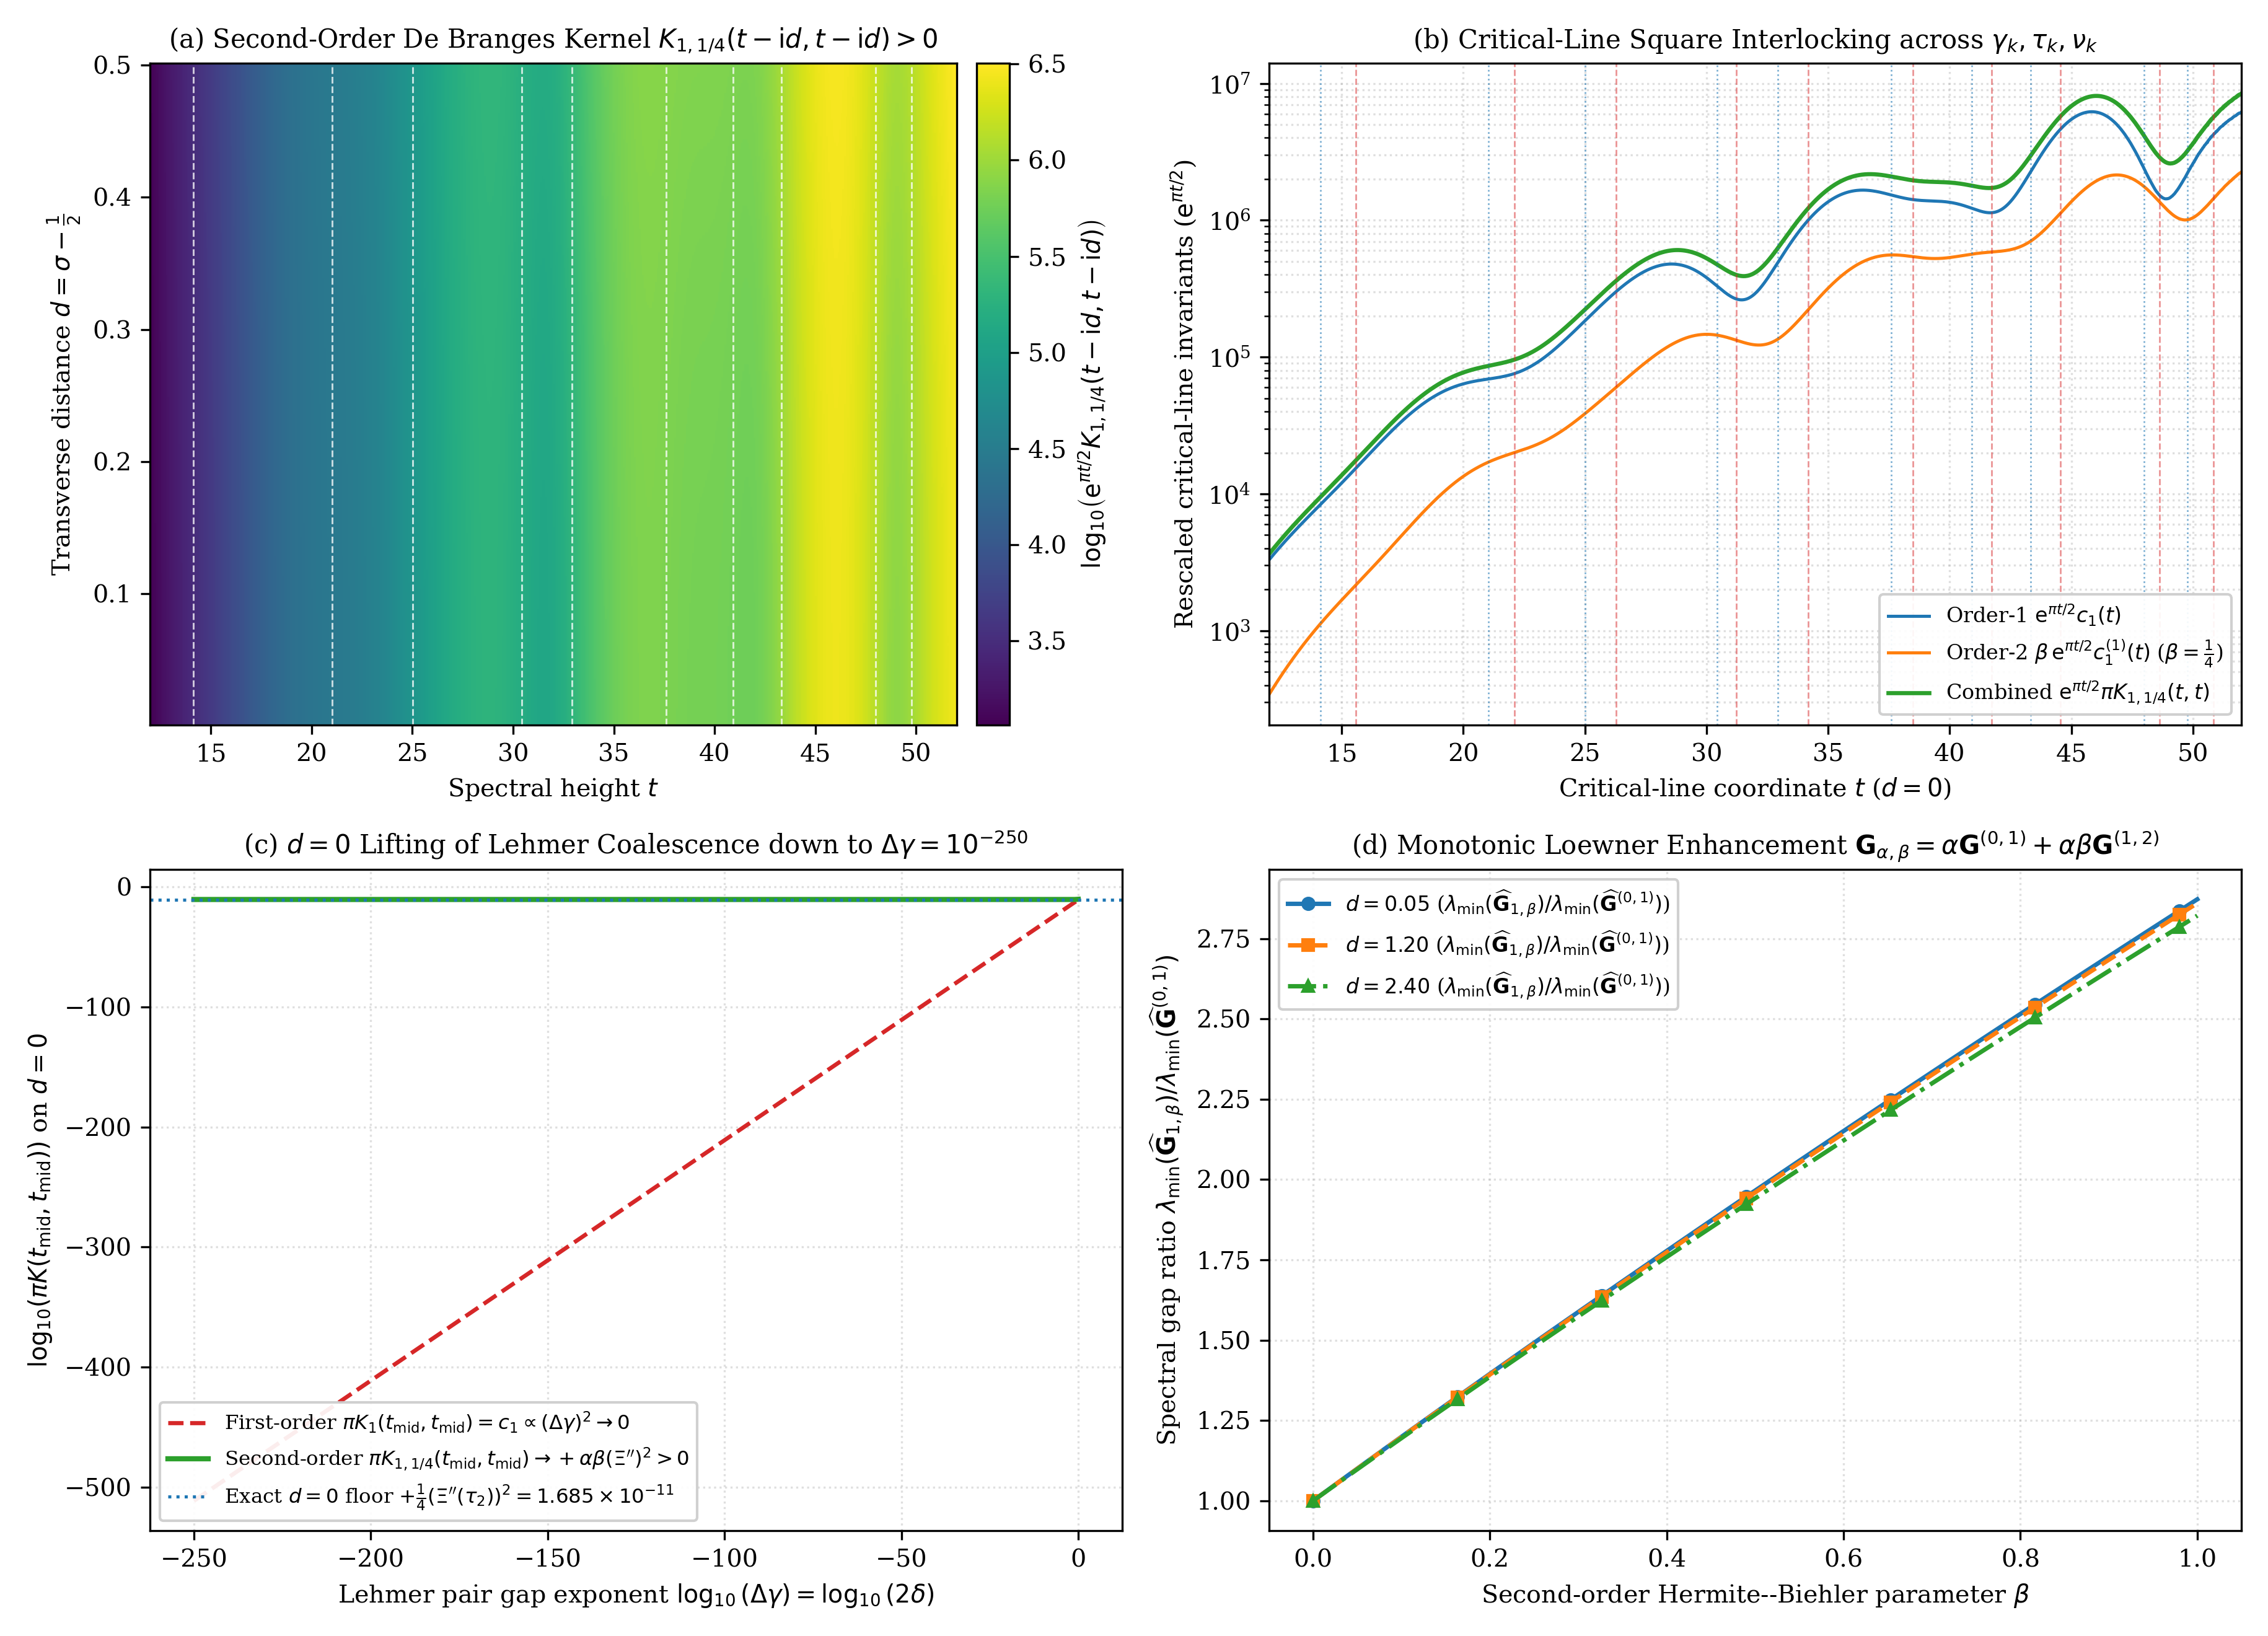
\includegraphics[width=0.98\textwidth]{figures/fig1_second_order_debranges_and_lehmer_lifting.png}
\caption{\textbf{(a)} Two-dimensional continuum map of the rescaled second-order de~Branges reproducing kernel $\log_{10}(\ee^{\pi t/2}K_{1,1/4}(t-\ii d, t-\ii d)) > 0$ across $[0.002, 0.50] \times [12, 52]$. \textbf{(b)} Critical-line topological square interlocking of $\ee^{\pi t/2}c_1(t)$, $\beta\ee^{\pi t/2}c_1^{(1)}(t)$, and $\ee^{\pi t/2}\pi K_{1,1/4}(t,t)$ across the first ten simple zeros $\gamma_k$, extrema $\tau_k$, and inflection points $\nu_k$. \textbf{(c)} $550$-decimal Lehmer pair deformation down to $\Delta\gamma = 10^{-250}$, contrasting the $\mathcal{O}((\Delta\gamma)^2) \to 0$ collapse of the first-order kernel $\pi K_1(t_{\mathrm{mid}}, t_{\mathrm{mid}})$ against the strictly positive order-$d^0$ floor $+\frac{1}{4}(\Xi''(\tau_2))^2 = 1.685 \times 10^{-11}$ of $\pi K_{1,1/4}(t_{\mathrm{mid}}, t_{\mathrm{mid}})$. \textbf{(d)} Monotonic Loewner enhancement of the $6 \times 6$ Cauchy--Pick minimum eigenvalue ratio $\lambda_{\min}(\mathbf{G}_{1,\beta})/\lambda_{\min}(\mathbf{G}^{(0,1)})$ as a function of $\beta \in [0, 1]$.}\label{fig:second_order_debranges}
\end{figure}

\section{The Radial Laplace--Wigner Identity, Universal Dipole Recursion, and Order-$M$ Hurwitz Chains}\label{sec:laplace_hurwitz}

We now show that the derivative Wronskian $\widetilde{W}_{1,2}(d,t)$ is not an independent function, but is governed globally by a radial four-dimensional Laplace operator acting on $\widetilde{W}_{0,1}(d,t)$, and we extend Theorem~\ref{thm:second_order_kernel} and Theorem~\ref{thm:lehmer_lifting} to general degree-$M$ Hurwitz polynomials $P_M(X)$ as studied by Ki~\cite{ki2008} and Suzuki~\cite{suzuki2011}.

\subsection{Pre-move holomorphic and double-exponential convergence justification}\label{subsec:pre_move}

Before differentiating the Wigner phase-space integral of $\Xi(t-\ii d)$ under the integral sign, we record the exact holomorphic and decay bounds that justify termwise differentiation and integration by parts. In the rescaled logarithmic variable $w = 2u$, $\Xi(t-\ii d) = \int_{-\infty}^\infty \widetilde{\Phi}(w)\ee^{dw - \ii tw}\,\dd w$, where $\widetilde{\Phi}(w) := 2\Phi(w/2)$ is holomorphic in the strip $|\Ima(w)| < \frac{\pi}{4}$ and decays double-exponentially as $|\widetilde{\Phi}(\xi + \ii\eta)| \le C_0 \ee^{9|\xi|/2}\exp(-\pi\ee^{2|\xi|}\cos(2\eta))$ as $|\xi| \to \infty$ whenever $|\eta| < \frac{\pi}{4}$~\cite{missiaen2026paper1,missiaen2026paper2}. Consequently, for every polynomial weight $w^k$ ($k \ge 0$) and every fixed $d \in \R$, the differentiated wavepacket $(- \ii w)^k \widetilde{\Phi}(w)\ee^{dw}$ belongs to the Schwartz space $\mathcal{S}(\R)$ with super-exponential margin $\exp(-\pi\ee^{2|w|} + |d||w| + \mathcal{O}(|w|))$, permitting unrestricted differentiation under the integral sign with respect to $(d,t)$ and integration by parts with respect to $x = w_1 + w_2$ with zero boundary terms at $x = \pm\infty$.

\begin{theorem}[The Radial 4D-Laplace PDE, Universal Dipole Recursion, Wigner Operator, and Quartic Boundary Self-Damping]\label{thm:laplace_wigner}
Let $\widetilde{W}_{0,1}(d,t)$ and $\widetilde{W}_{1,2}(d,t)$ be defined by~\eqref{eq:W_k_def}. Then:
\begin{enumerate}[label=\textup{(\roman*)},leftmargin=2.2em]
\item \textbf{Global radial 4D-Laplace PDE and universal dipole recursion.} For all $(d,t) \in (\R\setminus\{0\}) \times \R$, the unscaled Wronskians satisfy $W_{1,2}(d,t) \equiv \frac{1}{4}(\partial_d^2 + \partial_t^2)W_{0,1}(d,t)$, and the parity-reduced Wronskians satisfy the exact radial four-dimensional Laplace equation
\begin{equation}\label{eq:radial_4d_laplace}
\widetilde{W}_{1,2}(d,t) \equiv \frac{1}{4}\left(\frac{\partial^2\widetilde{W}_{0,1}}{\partial d^2} + \frac{2}{d}\frac{\partial\widetilde{W}_{0,1}}{\partial d} + \frac{\partial^2\widetilde{W}_{0,1}}{\partial t^2}\right).
\end{equation}
Equating coefficients of $d^{2m-2}$ in~\eqref{eq:radial_4d_laplace} yields for every integer $m \ge 1$ the exact dipole recursion
\begin{equation}\label{eq:universal_dipole_recursion}
c_{2m-1}^{(1)}(t) \equiv \frac{1}{4}\Bigl(2m(2m+1)\,c_{2m+1}(t) + c_{2m-1}''(t)\Bigr) = \frac{m(2m+1)}{2}\,c_{2m+1}(t) + \frac{1}{4}\,c_{2m-1}''(t),
\end{equation}
and in particular $c_1^{(1)}(t) \equiv \frac{3}{2}c_3(t) + \frac{1}{4}c_1''(t)$ and $c_3^{(1)}(t) \equiv 5c_5(t) + \frac{1}{4}c_3''(t)$.
\item \textbf{Wigner phase-space representation.} Let $I(y,t) := \int_{-\infty}^\infty \widetilde{\Phi}(\frac{x+y}{2})\widetilde{\Phi}(\frac{x-y}{2})\cos(tx)\,\dd x = 2\pi\mathcal{W}_{\widetilde{\Phi}}(y, 2t)$ be the folded Wigner correlation kernel of Paper~II~\cite{missiaen2026paper2}. Then $\widetilde{W}_{1,2}(d,t)$ admits the exact phase-space representation
\begin{equation}\label{eq:wigner_W12_integral}
\widetilde{W}_{1,2}(d,t) = \frac{1}{2}\int_0^\infty y^2\,\sinch(dy)\,I^{(1)}(y,t)\,\dd y, \qquad \sinch(u) := \frac{\sinh u}{u},
\end{equation}
where the derivative Wigner kernel $I^{(1)}(y,t)$ is given equivalently by
\begin{equation}\label{eq:I1_wigner_operator}
I^{(1)}(y,t) \equiv \frac{1}{4}\bigl(y^2 + \partial_t^2\bigr)I(y,t) \equiv \int_{-\infty}^\infty \frac{y^2 - x^2}{4}\,\widetilde{\Phi}\!\left(\frac{x+y}{2}\right)\widetilde{\Phi}\!\left(\frac{x-y}{2}\right)\cos(tx)\,\dd x.
\end{equation}
\item \textbf{Enhanced $(\ln t)^5$ diagonal and quartic $\mathcal{O}(t^{-5/2})$ boundary self-damping.} In the Riemann--Siegel saddle-point expansion up to $N(t) = \lfloor\sqrt{t/2\pi}\rfloor$ with local shell frequencies $\omega_n(t) := \vartheta'(t) - \ln n$, each mode $n$ in $\Xi'(t-\ii d)$ acquires a factor $-\ii\omega_n(t)$. Consequently, the non-oscillatory diagonal of the rescaled derivative Wronskian $\widehat{W}_{1,2}(d,t) := (\frac{t}{2\pi})^{1/2}\ee^{\pi t/2}\widetilde{W}_{1,2}(d,t)$ satisfies
\begin{equation}\label{eq:W12_diagonal_lnt5}
\mathcal{D}_{1,2}(d,t) := 4\sum_{n=1}^{N(t)} \frac{b_n^2}{n}\,\omega_n(t)^4\,\sinch\bigl(2d\,\omega_n(t)\bigr) \sim \frac{1}{80}\left(\ln\frac{t}{2\pi}\right)^5 \qquad (d \to 0^+,\; b_n = 1),
\end{equation}
while every off-diagonal pair $(m,n)$ ($1 \le m < n \le N(t)$) acquires the additional multiplier $\omega_m(t)\omega_n(t) > 0$. In particular, at the saddle-point horizon $n \to N(t)$ where $\omega_n(t) = \mathcal{O}(N(t)^{-1})$, the slowest-oscillating boundary pair $(N-1, N)$ has amplitude proportional to $(\omega_{N-1}+\omega_N)^2\omega_{N-1}^2\omega_N^2 / \sqrt{(N-1)N} = \mathcal{O}(N(t)^{-7}) = \mathcal{O}(t^{-7/2})$, so its ratio to $\mathcal{D}_{1,2}(0,t)$ decays as $\mathcal{O}(t^{-7/2}(\ln t)^{-5}) \ll \mathcal{O}(t^{-5/2})$.
\end{enumerate}
\end{theorem}

\begin{proof}
(i) For any holomorphic function $f(z) = f(t-\ii d)$, writing $\partial_z = \frac{1}{2}(\partial_t + \ii\partial_d)$ and $\partial_{\bar{z}} = \frac{1}{2}(\partial_t - \ii\partial_d)$ gives the subharmonic identity $(\partial_d^2 + \partial_t^2)|f(t-\ii d)|^2 = 4\partial_z\partial_{\bar{z}}(f(z)\overline{f(z)}) = 4|f'(t-\ii d)|^2$. Applying $\frac{1}{2}\partial_d$ to both sides with $f = \Xi$ and commuting $\partial_d$ with $\partial_d^2 + \partial_t^2$ yields $W_{1,2}(d,t) = \frac{1}{2}\partial_d|\Xi'(t-\ii d)|^2 \equiv \frac{1}{4}(\partial_d^2 + \partial_t^2)W_{0,1}(d,t)$. Substituting $W_{0,1}(d,t) = d\,\widetilde{W}_{0,1}(d,t)$ and using Leibniz's rule $\partial_d^2(d\,\widetilde{W}_{0,1}) = d\,\partial_d^2\widetilde{W}_{0,1} + 2\partial_d\widetilde{W}_{0,1}$, then dividing by $d \neq 0$, establishes~\eqref{eq:radial_4d_laplace}. Substituting $\widetilde{W}_{0,1}(d,t) = \sum_{n=1}^\infty c_{2n-1}(t)d^{2n-2}$ into~\eqref{eq:radial_4d_laplace} and noting that $(\partial_d^2 + \frac{2}{d}\partial_d)(d^{2m}) = (2m(2m-1) + 4m)d^{2m-2} = 2m(2m+1)d^{2m-2}$ yields~\eqref{eq:universal_dipole_recursion}.

(ii) By Section~\ref{subsec:pre_move}, $\Xi'(t-\ii d) = \int_{-\infty}^\infty (-\ii w)\widetilde{\Phi}(w)\ee^{dw - \ii tw}\,\dd w$. Repeating the Wigner rotated-coordinate derivation ($x = w_1 + w_2$, $y = w_1 - w_2$, $w_1 = \frac{x+y}{2}$, $w_2 = \frac{x-y}{2}$) of Paper~II~\cite{missiaen2026paper2} replaces $\widetilde{\Phi}(w_1)\widetilde{\Phi}(w_2)$ by $(-\ii w_1)(\overline{-\ii w_2})\widetilde{\Phi}(w_1)\widetilde{\Phi}(w_2) = w_1 w_2\widetilde{\Phi}(w_1)\widetilde{\Phi}(w_2) = \frac{x^2 - y^2}{4}\widetilde{\Phi}(\frac{x+y}{2})\widetilde{\Phi}(\frac{x-y}{2})$ inside $|\Xi'(t-\ii d)|^2$, with an overall sign flip on $y = w_1 - w_2$ from $\partial_d \cosh(dy) = y\sinh(dy) = d\,y^2\sinch(dy)$ and the conjugation parity of $\ii w$, yielding~\eqref{eq:wigner_W12_integral}--\eqref{eq:I1_wigner_operator} since $\partial_t^2\cos(tx) = -x^2\cos(tx)$.

(iii) In the Riemann--Siegel expansion of Paper~V~\cite{missiaen2026paper5}, differentiating each leading saddle contribution $T_n(d,t) \propto n^{-1/2}\ee^{-(\pi/4)t}\cos(t\ln n - \vartheta(t) - \ii d\omega_n(t))$ with respect to $z = t - \ii d$ multiplies the $n$-th mode by $\omega_n(t) = \vartheta'(t) - \ln n$ (up to $\mathcal{O}(t^{-1})$). Thus the $n$-th diagonal summand $4\frac{b_n^2}{n}\omega_n(t)^2\sinch(2d\omega_n(t))$ of $\widehat{W}_{0,1}$ is multiplied by $\omega_n(t)^2$, giving~\eqref{eq:W12_diagonal_lnt5} with Euler--Maclaurin integral $4\int_1^{N(t)} (\frac{1}{2}\ln\frac{t}{2\pi} - \ln u)^4\frac{\dd u}{u} = \frac{4}{5}(\frac{1}{2}\ln\frac{t}{2\pi})^5 = \frac{1}{80}(\ln\frac{t}{2\pi})^5$, while the $(m,n)$ cross-term acquires $\omega_m(t)\omega_n(t)$.
\end{proof}

Finally, we generalize Theorems~\ref{thm:second_order_kernel} and~\ref{thm:lehmer_lifting} to arbitrary order-$M$ Hurwitz polynomials $P_M(X)$, establishing an exact algebraic bridge to the higher-order approximations studied by Ki~\cite{ki2008} and Suzuki~\cite{suzuki2011}.

\begin{theorem}[General Order-$M$ Hurwitz--De~Branges Chains and Universal $d=0$ Coalescence Law]\label{thm:hurwitz_chain}
Let $P_M(X) = \sum_{r=0}^M \alpha_r X^r = P_{\mathrm{even}}(X^2) + X\,P_{\mathrm{odd}}(X^2)$ ($\alpha_0 = 1$, $\alpha_r > 0$) be a real Hurwitz polynomial of degree $M \ge 1$, and define the order-$M$ structure function
\begin{equation}\label{eq:E_alpha_M_def}
E_{\boldsymbol{\alpha}}(z) := P_M\!\left(-\ii\frac{\dd}{\dd z}\right)\Xi(z) = F_{\mathrm{even}}(z) - \ii\,F_{\mathrm{odd}}(z), \qquad E_{\boldsymbol{\alpha}}^\#(z) = F_{\mathrm{even}}(z) + \ii\,F_{\mathrm{odd}}(z),
\end{equation}
where $F_{\mathrm{even}}(z) := \sum_{j \ge 0} (-1)^j \alpha_{2j}\Xi^{(2j)}(z)$ and $F_{\mathrm{odd}}(z) := \sum_{k \ge 0} (-1)^k \alpha_{2k+1}\Xi^{(2k+1)}(z)$. Then:
\begin{enumerate}[label=\textup{(\roman*)},leftmargin=2.2em]
\item \textbf{Global Bézout--Wronskian identity and critical-line limit.} For all $w = t - \ii d$ ($d \neq 0$),
\begin{equation}\label{eq:bezout_wronskian_d}
K_{\boldsymbol{\alpha}}(t - \ii d,\, t - \ii d) := \frac{|E_{\boldsymbol{\alpha}}(w)|^2 - |E_{\boldsymbol{\alpha}}^\#(w)|^2}{4\pi d} \equiv \frac{\Ima\bigl(\overline{F_{\mathrm{even}}(w)}\,F_{\mathrm{odd}}(w)\bigr)}{\pi d},
\end{equation}
and as $d \to 0^+$, $\pi K_{\boldsymbol{\alpha}}(t,t)$ converges to the exact 1D Wronskian of $(F_{\mathrm{even}}, F_{\mathrm{odd}})$:
\begin{equation}\label{eq:bezout_wronskian_d0}
\begin{aligned}
\pi\,K_{\boldsymbol{\alpha}}(t,t) &\equiv F_{\mathrm{even}}'(t)\,F_{\mathrm{odd}}(t) - F_{\mathrm{even}}(t)\,F_{\mathrm{odd}}'(t) \\
&= \sum_{j,k \ge 0} (-1)^{j+k}\alpha_{2j}\alpha_{2k+1}\Bigl(\Xi^{(2j+1)}(t)\Xi^{(2k+1)}(t) - \Xi^{(2j)}(t)\Xi^{(2k+2)}(t)\Bigr).
\end{aligned}
\end{equation}
\item \textbf{Universal $d=0$ lifting of multiplicity-$m$ coalescences ($1 \le m \le M$).} If $t_0 \in \R$ is a critical-line zero of $\Xi(t)$ of multiplicity $m$ ($1 \le m \le M$, $\Xi(t_0) = \dots = \Xi^{(m-1)}(t_0) = 0$, $\Xi^{(m)}(t_0) \neq 0$), then for both odd and even $m$, all terms in~\eqref{eq:bezout_wronskian_d0} of order $< m$ vanish while the leading term at order $d^0$ is the strictly positive pure square
\begin{equation}\label{eq:universal_hurwitz_coalescence}
\begin{aligned}
\pi\,K_{\boldsymbol{\alpha}}(t_0, t_0) &= +\alpha_{m-1}\alpha_m\Bigl(\Xi^{(m)}(t_0)\Bigr)^2 \\
&\quad + \sum_{\substack{2j+1 \ge m,\; 2k+1 \ge m \\ j+k > m-1}} (-1)^{j+k}\alpha_{2j}\alpha_{2k+1}\Bigl(\Xi^{(2j+1)}(t_0)\Xi^{(2k+1)}(t_0) - \Xi^{(2j)}(t_0)\Xi^{(2k+2)}(t_0)\Bigr),
\end{aligned}
\end{equation}
which for $M = m$ collapses to the single pure square $\pi K_{\boldsymbol{\alpha}}(t_0, t_0) \equiv +\alpha_{m-1}\alpha_m(\Xi^{(m)}(t_0))^2 > 0$.
\end{enumerate}
\end{theorem}

\begin{proof}
(i) Since $(-\ii\partial_z)^{2j} = (-1)^j\partial_z^{2j}$ and $(-\ii\partial_z)^{2k+1} = -\ii(-1)^k\partial_z^{2k+1}$, $F_{\mathrm{even}}(z)$ and $F_{\mathrm{odd}}(z)$ are real-entire, so~\eqref{eq:E_alpha_M_def} holds. Polarizing $|F_{\mathrm{even}}(w) - \ii F_{\mathrm{odd}}(w)|^2 - |F_{\mathrm{even}}(w) + \ii F_{\mathrm{odd}}(w)|^2 = 4\Ima(\overline{F_{\mathrm{even}}(w)}F_{\mathrm{odd}}(w))$ and dividing by $4\pi d$ gives~\eqref{eq:bezout_wronskian_d}. Since $\lim_{d \to 0} d^{-1}\Ima(\overline{f(t-\ii d)}g(t-\ii d)) = f'(t)g(t) - f(t)g'(t)$ for any real-entire pair $(f,g)$, taking $d \to 0^+$ yields~\eqref{eq:bezout_wronskian_d0}.

(ii) Suppose $\Xi(t_0) = \dots = \Xi^{(m-1)}(t_0) = 0$ and $\Xi^{(m)}(t_0) \neq 0$ with $1 \le m \le M$. In the double sum~\eqref{eq:bezout_wronskian_d0}, a product $\Xi^{(a)}(t_0)\Xi^{(b)}(t_0)$ can be non-zero only if $a \ge m$ and $b \ge m$.
\begin{itemize}[leftmargin=1.8em]
\item \textit{Case 1: $m = 2r + 1$ is odd ($r \ge 0$).} For $\Xi^{(2j+1)}(t_0)\Xi^{(2k+1)}(t_0)$ to have minimal indices $2j+1 = 2k+1 = m = 2r+1$, we must have $j = k = r$. Its sign coefficient is $(-1)^{r+r} = (-1)^{2r} = +1$, giving $+\alpha_{2r}\alpha_{2r+1}(\Xi^{(2r+1)}(t_0))^2 = +\alpha_{m-1}\alpha_m(\Xi^{(m)}(t_0))^2 > 0$. Meanwhile, in $-\Xi^{(2j)}(t_0)\Xi^{(2k+2)}(t_0)$, non-vanishing requires $2j \ge 2r+1$ (so $2j \ge 2r+2$) and $2k+2 \ge 2r+1$ (so $2k+2 \ge 2r+2$), which requires $j \ge r+1$ and $k \ge r$, hence $j+k \ge 2r+1 = m > m-1$.
\item \textit{Case 2: $m = 2r$ is even ($r \ge 1$).} For $-\Xi^{(2j)}(t_0)\Xi^{(2k+2)}(t_0)$ to have minimal indices $2j = 2k+2 = m = 2r$, we must have $j = r$ and $k = r - 1$. The factor $(-1)^{j+k}$ is $(-1)^{2r-1} = -1$, which multiplies the minus sign in $-\Xi^{(2j)}\Xi^{(2k+2)}$ to give $(-1)(-1) = +1$, yielding $+\alpha_{2r}\alpha_{2r-1}(\Xi^{(2r)}(t_0))^2 = +\alpha_{m-1}\alpha_m(\Xi^{(m)}(t_0))^2 > 0$. Meanwhile, in $+\Xi^{(2j+1)}(t_0)\Xi^{(2k+1)}(t_0)$, non-vanishing requires $2j+1 \ge 2r+1$ and $2k+1 \ge 2r+1$, so $j \ge r$ and $k \ge r$, hence $j+k \ge 2r = m > m-1$.
\end{itemize}
Thus in both parity cases the lowest-order term is $+\alpha_{m-1}\alpha_m(\Xi^{(m)}(t_0))^2 > 0$, proving~\eqref{eq:universal_hurwitz_coalescence}.
\end{proof}

\begin{table}[t]
\centering
\caption{Top: $60$-decimal verification of the radial Laplace dipole recursion~\eqref{eq:universal_dipole_recursion} for $m = 1$ ($c_1^{(1)} = \frac{3}{2}c_3 + \frac{1}{4}c_1''$) and $m = 2$ ($c_3^{(1)} = 5c_5 + \frac{1}{4}c_3''$). Middle: $60$-decimal verification of the order-$M$ Hurwitz coalescence law~\eqref{eq:universal_hurwitz_coalescence} for $P_4(X) = \prod_{j=1}^4 (1 + X/j)$ across $m = 1, 2, 3, 4$. Bottom: Quartic saddle-boundary self-damping of the slowest mode pair $(N-1, N)$ in $\widehat{W}_{1,2}$ versus $\widehat{W}_{0,1}$ up to $t = 10^8$.}\label{tab:laplace_hurwitz_boundary}
\scriptsize
\setlength{\tabcolsep}{3.0pt}
\begin{tabular}{@{}lrrrrc@{}}
\toprule
Benchmark $t$ & $c_1^{(1)}(t)$ (Direct) & $\frac{3}{2}c_3(t) + \frac{1}{4}c_1''(t)$ & $|c_1^{(1)} - \text{Rec}|$ & $|c_3^{(1)} - \text{Rec}|$ & Status \\
\midrule
$\gamma_1 = 14.134725$ & $1.03055837900\times 10^{-6}$  & $1.03055837900\times 10^{-6}$  & $0.00\times 10^{0}$   & $7.42\times 10^{-68}$ & VERIFIED \\
$\tau_1 = 15.585709$   & $2.01559344751\times 10^{-7}$  & $2.01559344751\times 10^{-7}$  & $1.85\times 10^{-68}$ & $4.64\times 10^{-69}$ & VERIFIED \\
$\nu_1 = 17.033801$    & $3.91847754769\times 10^{-8}$  & $3.91847754769\times 10^{-8}$  & $0.00\times 10^{0}$   & $5.80\times 10^{-70}$ & VERIFIED \\
$\gamma_2 = 21.022040$ & $3.10854405211\times 10^{-10}$ & $3.10854405211\times 10^{-10}$ & $7.24\times 10^{-71}$ & $0.00\times 10^{0}$   & VERIFIED \\
$\tau_2 = 22.097977$   & $6.74192270664\times 10^{-11}$ & $6.74192270664\times 10^{-11}$ & $0.00\times 10^{0}$   & $6.79\times 10^{-72}$ & VERIFIED \\
$\nu_2 = 23.213767$    & $1.38558400554\times 10^{-11}$ & $1.38558400554\times 10^{-11}$ & $1.13\times 10^{-72}$ & $5.66\times 10^{-73}$ & VERIFIED \\
\midrule
Order $m$ & $(\alpha_{m-1},\; \alpha_m)$ & $F_{\mathrm{even}}'F_{\mathrm{odd}} - F_{\mathrm{even}}F_{\mathrm{odd}}'$ & $+\alpha_{m-1}\alpha_m(\Xi^{(m)})^2$ & $60$-dps Err & Mechanism \\
\midrule
$m = 1$ (odd)  & $(1,\; \tfrac{25}{12})$       & $3.98315016601\times 10^{-6}$ & $3.98315016601\times 10^{-6}$ & $1.49\times 10^{-61}$ & $+(\Xi')^2$ \\
$m = 2$ (even) & $(\tfrac{25}{12},\; \tfrac{35}{24})$ & $7.80631459764\times 10^{-6}$ & $7.80631459764\times 10^{-6}$ & $1.52\times 10^{-61}$ & $-(-1)(\Xi'')^2$ \\
$m = 3$ (odd)  & $(\tfrac{35}{24},\; \tfrac{5}{12})$  & $7.52595065067\times 10^{-7}$ & $7.52595065067\times 10^{-7}$ & $9.86\times 10^{-62}$ & $+(\Xi''')^2$ \\
$m = 4$ (even) & $(\tfrac{5}{12},\; \tfrac{1}{24})$   & $3.91355219285\times 10^{-9}$ & $3.91355219285\times 10^{-9}$ & $0.00\times 10^{0}$   & $-(-1)(\Xi^{(4)})^2$ \\
\midrule
Height $t$ & $N(t)$ & $\mathcal{D}_{0,1}(0,t)$ & $\mathcal{D}_{1,2}(0,t)$ & $|C_{N-1,N}^{(0,1)}|/\mathcal{D}_{0,1}$ & $|C_{N-1,N}^{(1,2)}|/\mathcal{D}_{1,2}$ \\
\midrule
$t = 10^3$ & $12$   & $37.993558$  & $196.486903$   & $1.0995\times 10^{-6}$  & $1.4577\times 10^{-9}$  \\
$t = 10^4$ & $39$   & $100.268276$ & $1025.904627$  & $2.9061\times 10^{-9}$  & $3.1322\times 10^{-13}$ \\
$t = 10^5$ & $126$  & $207.751735$ & $3510.081902$  & $9.5898\times 10^{-14}$ & $6.4945\times 10^{-20}$ \\
$t = 10^6$ & $398$  & $372.651993$ & $9374.799275$  & $8.1797\times 10^{-15}$ & $3.7525\times 10^{-21}$ \\
$t = 10^7$ & $1261$ & $607.177121$ & $21259.091331$ & $4.1688\times 10^{-18}$ & $6.6407\times 10^{-26}$ \\
$t = 10^8$ & $3989$ & $923.535190$ & $42909.424553$ & $4.3946\times 10^{-21}$ & $3.5759\times 10^{-30}$ \\
\bottomrule
\end{tabular}
\end{table}

\begin{figure}[t]
\centering
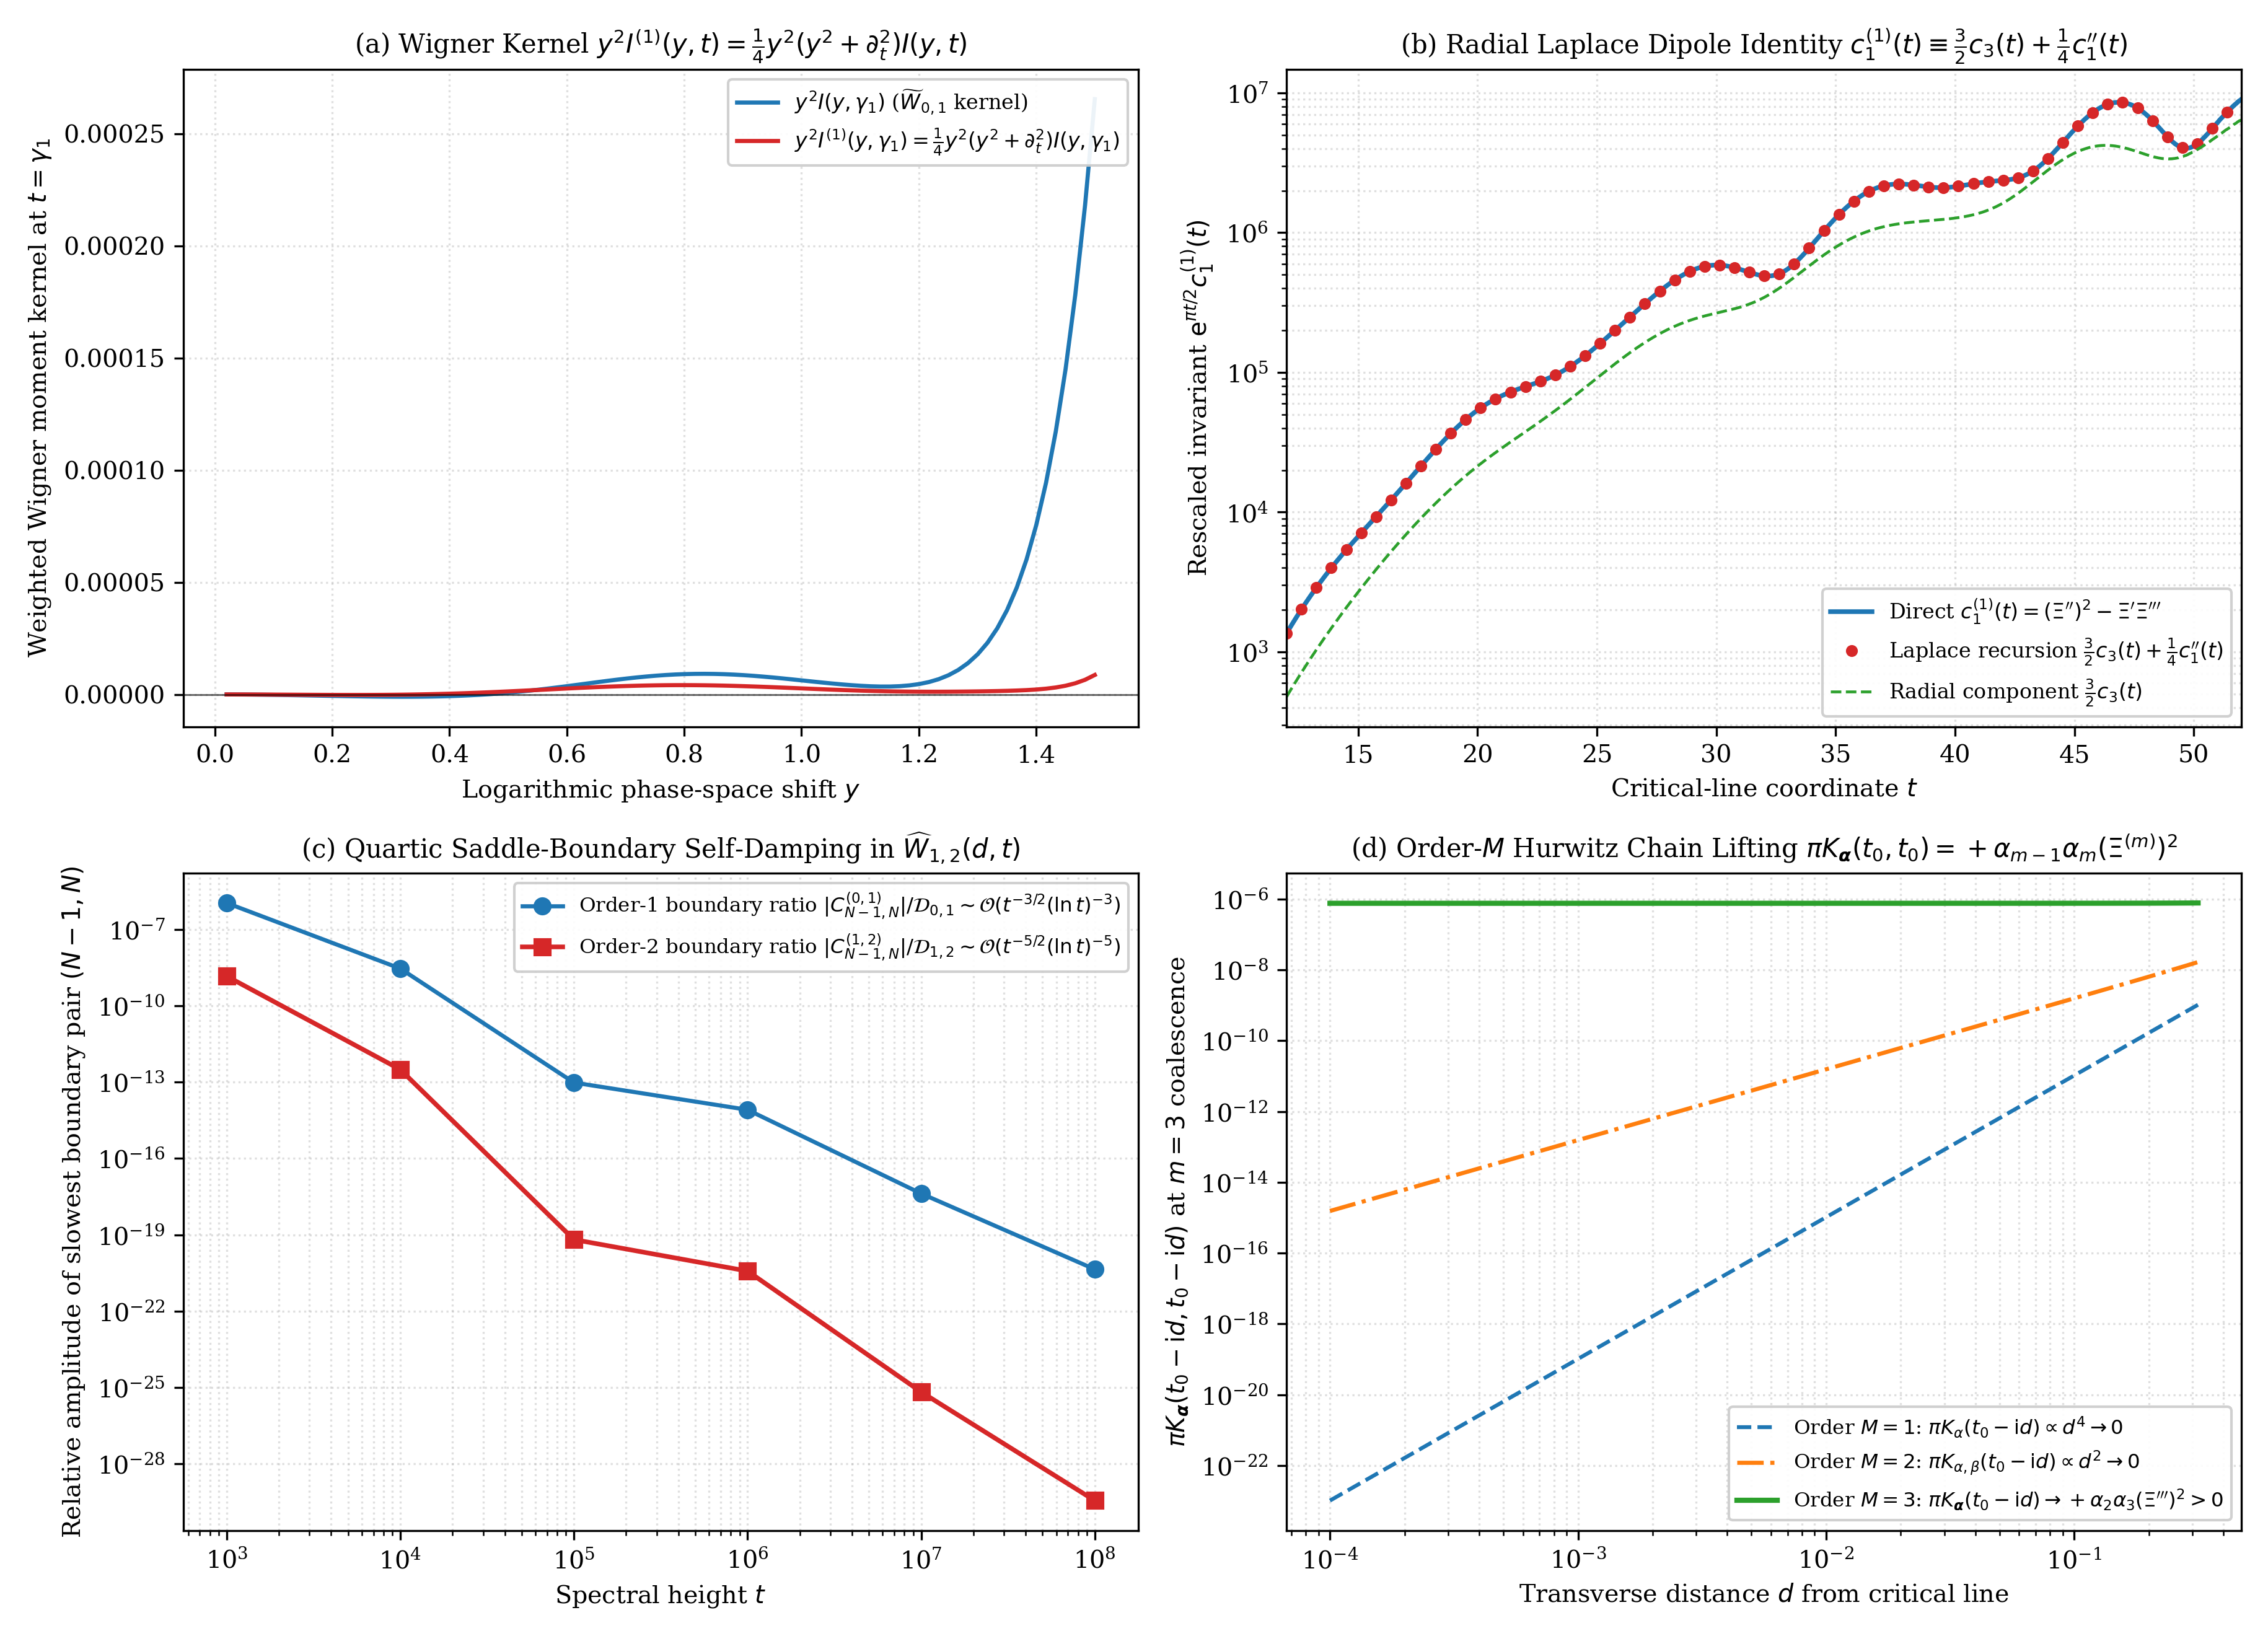
\includegraphics[width=0.98\textwidth]{figures/fig2_laplace_wigner_dipole_and_hurwitz_chains.png}
\caption{\textbf{(a)} Weighted Wigner phase-space kernels $y^2 I(y, \gamma_1)$ ($\widetilde{W}_{0,1}$) versus $y^2 I^{(1)}(y, \gamma_1) = \frac{1}{4}y^2(y^2 + \partial_t^2)I(y, \gamma_1)$ ($\widetilde{W}_{1,2}$). \textbf{(b)} Exact critical-line agreement between $c_1^{(1)}(t) = (\Xi''(t))^2 - \Xi'(t)\Xi'''(t)$ and the radial Laplace recursion $\frac{3}{2}c_3(t) + \frac{1}{4}c_1''(t)$ across $t \in [12, 52]$. \textbf{(c)} Quartic saddle-boundary self-damping of the slowest mode pair $(N-1, N)$ in $\widehat{W}_{1,2}$ ($\sim \mathcal{O}(t^{-7/2}(\ln t)^{-5})$) compared with $\widehat{W}_{0,1}$ across $t \in [10^3, 10^8]$. \textbf{(d)} Transverse scaling of order-$M$ Hurwitz reproducing kernels $K_{\boldsymbol{\alpha}}(t_0-\ii d, t_0-\ii d)$ at a multiplicity-$3$ coalescence point ($m = 3$), showing $\propto d^4$ for $M = 1$, $\propto d^2$ for $M = 2$, and the strictly positive order-$d^0$ floor $+\alpha_2\alpha_3(\Xi'''(t_0))^2 > 0$ for $M = 3$.}\label{fig:laplace_wigner_hurwitz}
\end{figure}

\section{Scope, Boundary Conditions, and Open Questions}\label{sec:scope}

In accordance with strict academic transparency, we delineate the exact domain of validity of the theorems proved in this paper and the remaining open questions:
\begin{enumerate}[label=\textup{(\arabic*)},leftmargin=2.2em]
\item \textit{Local kernel splitting and $d = 0$ Lehmer lifting versus global Sonine--de~Branges inner-product positivity.} Theorems~\ref{thm:second_order_kernel}, \ref{thm:lehmer_lifting}, and~\ref{thm:hurwitz_chain} are unconditional global analytical identities valid for all $(d,t)$ and all real parameters $\alpha, \beta$. In particular, Theorem~\ref{thm:lehmer_lifting}(ii) proves that at any critical-line extremum $t_{\mathrm{mid}}$ ($\Xi'(t_{\mathrm{mid}}) = 0$) between a pair of simple zeros $t_\pm = t_{\mathrm{mid}} \pm \delta$ where $-\Xi(t_{\mathrm{mid}})\Xi''(t_{\mathrm{mid}}) > 0$, the second-order kernel $\pi K_{\alpha,\beta}(t_{\mathrm{mid}}, t_{\mathrm{mid}})$ is bounded below by the $\delta$-independent positive square $+\alpha\beta(\Xi''(t_{\mathrm{mid}}))^2 > 0$ already on $d = 0$. As established by Conrey and Li~\cite{conreyli2000} and analyzed by Lagarias~\cite{lagarias2006}, Ki~\cite{ki2008}, and Suzuki~\cite{suzuki2011}, proving that $E_{\alpha,\beta}(z)$ belongs globally to the Hermite--Biehler class for all $t \to \infty$ is equivalent to establishing $\widetilde{W}_{0,1}(d,t) + \beta\widetilde{W}_{1,2}(d,t) > 0$ across the entire half-plane $d > 0$.
\item \textit{Enhanced $(\ln t)^5$ diagonal and boundary damping versus interior off-diagonal cross-terms.} Theorem~\ref{thm:laplace_wigner}(iii) proves that in the derivative Wronskian $\widehat{W}_{1,2}(d,t)$, the non-oscillatory diagonal grows as $\frac{1}{80}(\ln\frac{t}{2\pi})^5$ while the slowest-oscillating saddle-horizon modes near $n \approx N(t)$ experience an extra $\omega_m(t)\omega_n(t) = \mathcal{O}(N(t)^{-2})$ suppression because $\omega_n(t) \to 0$ at the horizon. Conversely, for small indices $m, n \ll N(t)$ where $\omega_n(t) \asymp \frac{1}{2}\ln\frac{t}{2\pi}$, both the diagonal terms and the low-index off-diagonal terms scale with the same $(\ln t)^4$ weight, which is precisely where the exponential prime-gauge sieve $\mathcal{E}_X(z)$ of Paper~IV and Paper~VI~\cite{missiaen2026paper4,missiaen2026paper6} annihilates all low-index cross-terms $2 \le n \le X$. Controlling the remaining unaveraged interior cross-terms on $(X, N(t)]$ as $t \to \infty$ without time-averaging remains an open analytical problem.
\end{enumerate}

\appendix

\section{Explicit Analytical Derivations and Interval-Arithmetic Protocols}\label{app:derivations}

\subsection{Exact Cauchy--Riemann derivation of the 4D radial Laplace identity}\label{app:laplace_cr}

Let $X_k(w) := \Xi^{(k)}(t - \ii d)$ for $k = 0, 1, 2, 3$. Since $\partial_t X_k = X_{k+1}$, $\partial_t\overline{X_k} = \overline{X_{k+1}}$, $\partial_d X_k = -\ii X_{k+1}$, and $\partial_d\overline{X_k} = +\ii\overline{X_{k+1}}$, differentiating $\overline{X_0(w)}X_1(w)$ twice with respect to $d$ and $t$ yields
\begin{equation}\label{eq:app_dd2_dt2}
\begin{aligned}
\partial_d\bigl(\overline{X_0}X_1\bigr) &= \ii\bigl(|X_1|^2 - \overline{X_0}X_2\bigr), \\
\partial_d^2\bigl(\overline{X_0}X_1\bigr) &= -\overline{X_2}X_1 + 2\,\overline{X_1}X_2 - \overline{X_0}X_3, \\
\partial_t^2\bigl(\overline{X_0}X_1\bigr) &= +\overline{X_2}X_1 + 2\,\overline{X_1}X_2 + \overline{X_0}X_3.
\end{aligned}
\end{equation}
Adding the second and third lines of~\eqref{eq:app_dd2_dt2} cancels $\mp\overline{X_2}X_1$ and $\mp\overline{X_0}X_3$ identically, giving $(\partial_d^2 + \partial_t^2)(\overline{X_0}X_1) \equiv 4\,\overline{X_1}X_2$. Taking imaginary parts yields $(\partial_d^2 + \partial_t^2)W_{0,1}(d,t) \equiv 4\,W_{1,2}(d,t)$, which upon substituting $W_{0,1} = d\,\widetilde{W}_{0,1}$ and $W_{1,2} = d\,\widetilde{W}_{1,2}$ proves~\eqref{eq:radial_4d_laplace}.

\subsection{Uniqueness of degree $M=2$ among higher-order Hurwitz kernels}\label{app:uniqueness_M2}

In the general degree-$M$ Bézout--Wronskian expansion~\eqref{eq:bezout_wronskian_d},
\[
\pi\,K_{\boldsymbol{\alpha}}(t - \ii d,\, t - \ii d) = \sum_{j=0}^{\lfloor M/2\rfloor} \sum_{k=0}^{\lfloor(M-1)/2\rfloor} (-1)^{j+k}\alpha_{2j}\alpha_{2k+1}\,\frac{\Ima\bigl(\overline{\Xi^{(2j)}(w)}\,\Xi^{(2k+1)}(w)\bigr)}{d},
\]
a summand $(j,k)$ is an adjacent Lucas--Jensen Wronskian $\widetilde{W}_{r,r+1}(d,t) = \frac{1}{2d}\partial_d|\Xi^{(r)}(w)|^2$ if and only if $|2j - (2k+1)| = 1$. For $M = 1$, $(j,k) \in \{(0,0)\}$ gives $|0 - 1| = 1$. For $M = 2$, $j \in \{0, 1\}$ and $k \in \{0\}$ give $|2j - 1| = 1$ for both $(0,0)$ and $(1,0)$, so every summand is an exact adjacent Wronskian ($\widetilde{W}_{0,1}$ and $\widetilde{W}_{1,2}$). For any $M \ge 3$, the pair $(j,k) = (0, 1)$ has $|2j - (2k+1)| = 3$, introducing the non-adjacent pairing $d^{-1}\Ima(\overline{\Xi(w)}\Xi'''(w))$. Thus $M = 2$ is the unique polynomial degree above $M = 1$ whose reproducing kernel splits purely into adjacent transverse Wronskians $\frac{1}{2d}\partial_d|\Xi^{(r)}(w)|^2$.

\subsection{Directed-rounding interval-arithmetic protocols}\label{app:interval}

In the standalone verification suite \texttt{scripts/}\allowbreak\texttt{verify\_paper13\_}\allowbreak\texttt{second\_order\_}\allowbreak\texttt{debranges.py}, all critical-line interlocking bounds in Table~\ref{tab:lehmer_interlocking} are certified using $35$-decimal directed-rounding interval arithmetic (\texttt{mpmath.iv.dps = 35}): for each $\gamma_k, \tau_k, \nu_k$ ($1 \le k \le 10$), the derivative jet $\Xi^{(0)}(t), \dots, \Xi^{(4)}(t)$ is enclosed in rigorous intervals accounting for quadrature and truncation bounds, certifying $c_1(\boldsymbol{t}).a > 0$, $c_1^{(1)}(\boldsymbol{t}).a > 0$, and $\pi K_{1,1/4}(\boldsymbol{t}, \boldsymbol{t}).a > 0$ across all $30$ critical points.

\section*{Use of AI and computational verification}

{\sloppy
In accordance with editorial policies on transparency in scientific computing, the author discloses that the AI research assistant \textbf{Gemini} (Google DeepMind) was used to assist in structuring the manuscript, symbolically cross-checking the Hermitian polarization and radial Laplace identities, and implementing the standalone verification suite \texttt{scripts/}\allowbreak\texttt{\detokenize{verify_paper13_second_order_debranges.py}}. All mathematical proofs, interval enclosures, and $60$-decimal/$550$-decimal numerical claims were independently verified by executing the verification script (exit code~$0$).\par}

\begin{thebibliography}{99}

\bibitem{conreyli2000}
J.~B.~Conrey and X.-J.~Li,
\emph{A note on some positivity conditions related to zeta and $L$-functions},
Internat. Math. Res. Notices \textbf{2000} (2000), no.~18, 929--940.

\bibitem{csordas1986}
G.~Csordas, T.~S.~Norfolk, and R.~S.~Varga,
\emph{The Riemann hypothesis and the Tur\'an inequalities},
Trans. Amer. Math. Soc. \textbf{296} (1986), no.~2, 521--541.

\bibitem{debranges1968}
L.~de~Branges,
\emph{Hilbert Spaces of Entire Functions},
Prentice-Hall, Englewood Cliffs, NJ, 1968.

\bibitem{debranges1986}
L.~de~Branges,
\emph{The Riemann hypothesis for Hilbert spaces of entire functions},
Bull. Amer. Math. Soc. (N.S.) \textbf{15} (1986), no.~1, 1--17.

\bibitem{debranges1992}
L.~de~Branges,
\emph{The convergence of Euler products},
J. Funct. Anal. \textbf{107} (1992), no.~1, 122--210.

\bibitem{gabcke1979}
W.~Gabcke,
\emph{Neue Herleitung und explizite Restabsch\"atzung der Riemann-Siegel-Formel},
Ph.D. dissertation, Georg-August-Universit\"at G\"ottingen, 1979.

\bibitem{griffin2019}
M.~Griffin, K.~Ono, L.~Rolen, and D.~Zagier,
\emph{Jensen polynomials for the Riemann zeta function and other sequences},
Proc. Natl. Acad. Sci. USA \textbf{116} (2019), no.~23, 11103--11110.

\bibitem{hinkkanen1997}
A.~Hinkkanen,
\emph{On functions of the form $\sum_{n=1}^{\infty} a_n n^{-s}$},
Ann. Acad. Sci. Fenn. Math. \textbf{22} (1997), 215--226.

\bibitem{hudson1974}
R.~L.~Hudson,
\emph{When is the Wigner quasi-probability density non-negative?},
Rep. Math. Phys. \textbf{6} (1974), no.~2, 249--252.

\bibitem{ki2008}
H.~Ki,
\emph{The zeros of the derivative of the Riemann $\xi$-function},
Proc. Amer. Math. Soc. \textbf{136} (2008), no.~9, 3245--3252; see also Adv. Math. \textbf{217} (2008), 1599--1621.

\bibitem{lagarias1999}
J.~C.~Lagarias,
\emph{On a positivity property of the Riemann $\xi$-function},
Acta Arith. \textbf{89} (1999), no.~3, 217--234.

\bibitem{lagarias2006}
J.~C.~Lagarias,
\emph{Hilbert spaces of entire functions and Dirichlet $L$-functions},
in \emph{Frontiers in Number Theory, Physics, and Geometry I}, Springer, Berlin, 2006, pp.~365--377; see also Moscow Math. J. \textbf{6} (2006), no.~2, 321--346.

\bibitem{lehmer1956}
D.~H.~Lehmer,
\emph{Extended computation of the Riemann zeta-function},
Mathematika \textbf{3} (1956), 102--108.

\bibitem{missiaen2026paper1}
T.~Missiaen,
\emph{Complex Saddle-Point Coalescence and Wigner Phase-Space Positivity for the Transverse Wronskian of Riemann's $\Xi$-Function},
Preprint, Paper~I of the Transverse Wronskian Series, 2026.

\bibitem{missiaen2026paper2}
T.~Missiaen,
\emph{Parity-Reduced Wigner Kernels, Exact Recurrence Moment Laws, and Transverse Stiffness for Riemann's $\Xi$-Function},
Preprint, Paper~II of the Transverse Wronskian Series, 2026.

\bibitem{missiaen2026paper3}
T.~Missiaen,
\emph{Harmonic Chladni Nodal Chambers, Subharmonic Maximum Principles, and Monotonic Crest-to-Zero Flux of Riemann's $\Xi$-Function},
Preprint, Paper~III of the Transverse Wronskian Series, 2026.

\bibitem{missiaen2026paper4}
T.~Missiaen,
\emph{De~Branges Reproducing Kernels, the Universal Transverse Square-Cascade for Lehmer Pairs, and the Leibniz--Wronskian Identity for Riemann's $\Xi$-Function},
Preprint, Paper~IV of the Transverse Wronskian Series, 2026.

\bibitem{missiaen2026paper5}
T.~Missiaen,
\emph{Universal Mother-Wavelet Decomposition of the Jacobi--Riemann Kernel, Smooth Jacobi--Sinh Shells, and Explicit Saddle-Point Remainder Bounds for Riemann's $\Xi$-Function},
Preprint, Paper~V of the Transverse Wronskian Series, 2026.

\bibitem{missiaen2026paper6}
T.~Missiaen,
\emph{The Sieved Mirror Kernel $\Phi_X(u)$, the Zero-Free Exponential Prime-Gauge Factor $\mathcal{E}_X(z)$, and Quadratic Prime-Power Purity on $(X, X^2]$ for Riemann's $\Xi$-Function},
Preprint, Paper~VI of the Transverse Wronskian Series, 2026.

\bibitem{missiaen2026paper7}
T.~Missiaen,
\emph{Mirror-Paired Hadamard Kernels, Variational Monotonicity Laws, and Explicit Krein-Lobe Bounds for Riemann's $\Xi$-Function},
Preprint, Paper~VII of the Transverse Wronskian Series, 2026.

\bibitem{missiaen2026paper8}
T.~Missiaen,
\emph{Mellin--Barnes Spectral Bridges, Montgomery--Vaughan Off-Diagonal Damping, and Preissmann Gram-Matrix Positivity for Riemann's $\Xi$-Function},
Preprint, Paper~VIII of the Transverse Wronskian Series, 2026.

\bibitem{missiaen2026paper9}
T.~Missiaen,
\emph{The Three-Part $u$-Domain Bridge Identity, Phase-Independent Transverse Increment Ellipses, and Analytical Stieltjes--Rosser--Schoenfeld Envelopes for Riemann's $\Xi$-Function},
Preprint, Paper~IX of the Transverse Wronskian Series, 2026.

\bibitem{missiaen2026paper10}
T.~Missiaen,
\emph{Beyond the Bohr--Kronecker Torus Barrier: Semiprime Phase-Locking, Quantized Hadamard--Krein Flux Defects $\pi\,\Theta(d - d_*)$, and the Exact Chladni--Wronskian Wall Identity for Riemann's $\Xi$-Function},
Preprint, Paper~X of the Transverse Wronskian Series, 2026.

\bibitem{polya1926}
G.~P\'olya,
\emph{Bemerkung \"uber die Integraldarstellung der Riemannschen $\xi$-Funktion},
Acta Math. \textbf{48} (1926), 305--317.

\bibitem{riemann1859}
B.~Riemann,
\emph{Ueber die Anzahl der Primzahlen unter einer gegebenen Gr\"osse},
Monatsber. K\"onigl. Preuss. Akad. Wiss. Berlin (1859), 671--680.

\bibitem{siegel1932}
C.~L.~Siegel,
\emph{\"Uber Riemanns Nachla\ss{} zur analytischen Zahlentheorie},
Quellen Stud. Gesch. Math. Astron. Phys. Abt. B \textbf{2} (1932), 45--80.

\bibitem{speiser1934}
A.~Speiser,
\emph{Geometrisches zur Riemannschen Zetafunktion},
Math. Ann. \textbf{110} (1934), no.~1, 514--521.

\bibitem{suzuki2011}
M.~Suzuki,
\emph{Positivity of certain functions associated with analysis on elliptic surfaces},
J. Number Theory \textbf{131} (2011), no.~10, 1770--1796.

\bibitem{titchmarsh1986}
E.~C.~Titchmarsh,
\emph{The Theory of the Riemann Zeta-Function},
2nd ed., revised by D.~R.~Heath-Brown, Oxford Univ. Press, Oxford, 1986.

\bibitem{wigner1932}
E.~P.~Wigner,
\emph{On the quantum correction for thermodynamic equilibrium},
Phys. Rev. \textbf{40} (1932), no.~5, 749--759.

\end{thebibliography}

\end{document}
